\documentclass[a4paper]{article}
\usepackage[italian]{babel}
\usepackage[T1]{fontenc}
\usepackage[utf8]{inputenc}
\usepackage{graphicx}
\usepackage[margin=1in]{geometry}
\usepackage{makecell}
\usepackage[table]{xcolor}
\usepackage{setspace}
\usepackage{tabularx} 
\usepackage{hyperref}
\usepackage{array}
\usepackage{fancyhdr}
\usepackage{hyperref}
\usepackage{float}
\usepackage{bold-extra}

\usepackage{titlesec}

\setcounter{secnumdepth}{4}

\titleformat{\paragraph}
{\normalfont\normalsize\bfseries}{\theparagraph}{1em}{}
\titlespacing*{\paragraph}
{0pt}{3.25ex plus 1ex minus .2ex}{1.5ex plus .2ex}

\makeindex

\title{
	\textbf{BORA BORA FITNESS CLUB}\\
	\large Relazione di progetto di Tecnologie Web
}
\date{Anno 2021 - 2022}

\begin{document}
	\maketitle

	\begin{table}[H]
		\centering
		\begin{tabular}{c|l l}
			\textbf{Componenti}	& Adnan Latif Gazi			& 1224442\\
								& Alberto Lazari			& 1216747\\
								& Marco Andrea Limongelli	& 1225415\\
								& Francesco Protopapa		& 1221598\\
		\end{tabular}
	\end{table}


	
	\begin{table}[H]
		\centering
		\begin{tabular}{|l|l|l|}
			\hline
			\textbf{Tipologia di utente}	& \textbf{Username}	& \textbf{Password}\\
			\hline
			Utente generico					& user				& user\\
			\hline
			Utente amministratore			& admin				& admin\\
			\hline
		\end{tabular}
		\caption{Credenziali degli utenti del sito.}
	\end{table}

	\pagebreak

	% indice
	\renewcommand{\contentsname}{Indice}
	\tableofcontents
	\pagebreak

	\section{Introduzione}
	\subsection{Abstract}
	Il progetto Bora Bora Fitness Club, svolto come finalità del corso di Tecnologie Web nell'anno accademico 2021-2022, si propone di implementare un sito web per la gestione delle attività relativa ad una palestra. Il nome è ottenuto unendo i titoli dell'isola della polinesia francese di Bora Bora, in cui sorge l'attività, con una classica e indicativa denominazione delle palestre (Fitness Club).\\ 
	Esistono moltissimi siti relativi a palestre, ma praticamente tutte si limitano alla sola presentazione della propria impresa: Bora Bora Fitness Club invece mette a disposizione degli utilizzatori del sito le funzionalità che risultano essere le più desiderate dai clienti, quali la gestione dei propri allenamenti ed esercizi, interazione con gli allenamenti degli altri utenti, tracciamento delle proprie attività, gestione dei dati personali e abbonamenti.\\
	Per conseguire lo scopo, la natura del sito è fortemente interattiva, ma unisce anche una sostanziosa parte per la presentazione dell'impresa. Per i visitatori è infatti possibile accedere al proprio account, grazie al quale gestire le proprie attività di palestra. Nonostante ciò l'autenticazione non è obbligatoria: il visitatore ha comunque a disposizione tutte le funzionalità informative.\\
	Il sito è stato sviluppato con l'intenzione di essere poi pubblicato su Internet, dunque si è data molta importanza alla sua usabilità, rispettando gli standard W3C, la separazione tra struttura, presentazione, comportamento e le regole di accessibilità richieste.

	\subsection{Analisi dell'utenza}
	Il sito web si rivolge prevalentemente ad un pubblico di abitanti o visitatori dell'isola che intendono allenarsi nella sua unica palestra disponibile. Sebbene in minima parte, viene anche utilizzato dai gestori della palestra e una parte dei clienti degli alberghi convenzionati, che, pagando la quota di iscrizione una tantum alla palestra, hanno libero accesso al Bora Bora Fitness Club fintantoché pernottano nei resort.\\
	La palestra raccoglie pertanto una clientela relativamente al passo con la tecnologia, principalmente abbiente e solitamente giovane. Il sito risulta essere ottimizzato per la visualizzazione da telefono, in quanto è stato appurato che la maggior parte degli utenti salvino i propri allenamenti nel sito, e una volta arrivati in palestra si allenino seguendo la scheda degli esercizi direttamente dal telefono. Essendo che però potrebbe essere presente una piccola parte della clientela non aggiornata con le ultime tecnologie e non in grado di comprendere o utilizzare le funzionalità più moderne, il sito è stato realizzato garantendo l'usabilità delle sue funzioni a prescindere dal tipo di tecnologia e utente, nonostante diventi meno accattivante se usato con le tecnologie meno recenti.\\
	L'utenza target del sito si divide in 3 gruppi, una volta che visitano il sito:
	\begin{itemize}
		\item \textbf{Admin:} amministra sugli utenti e le loro attività in modo da regolare il corretto funzionamento del sito.
		\item \textbf{Utente registrato:} usufruisce delle funzionalità di gestione delle proprie attività in modo da godere della più ampia esperienza di palestra.
		\item \textbf{Utente non registrato:} ricerca informazioni da una panoramica della palestra al fine di valutare il suo interesse per la palestra.
		
	\end{itemize}

	\section{Progettazione}
	\subsection{Struttura del sito}
	\begin{figure}[H]
		\centering
		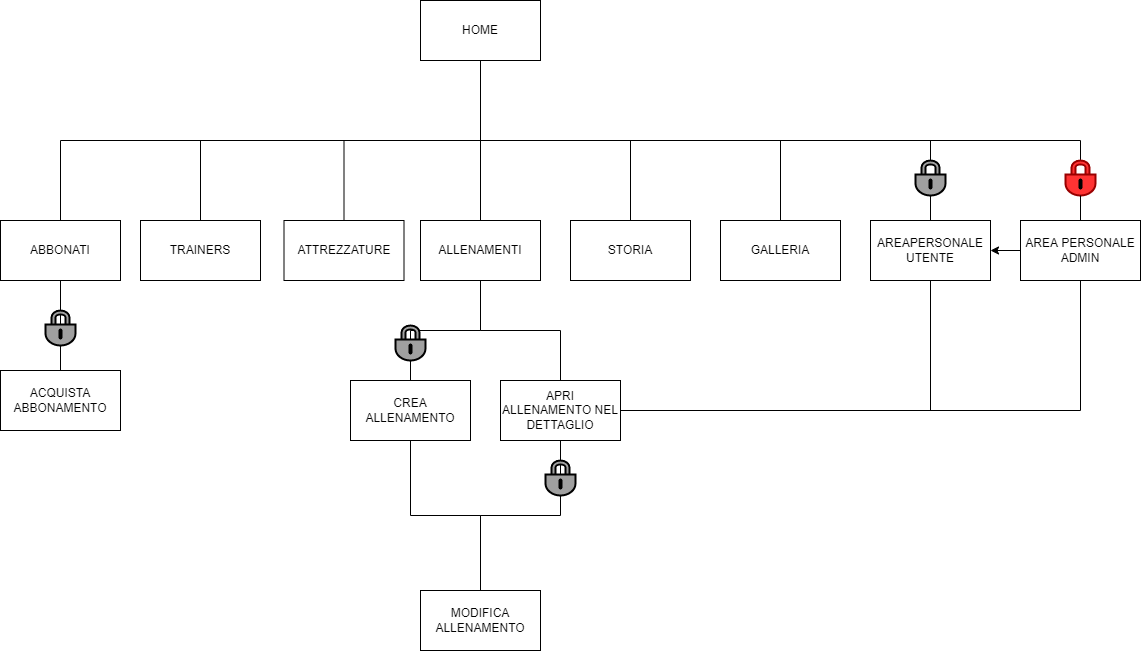
\includegraphics[scale=0.3]{immagini/mappa_sito.drawio.png}
		\caption{Mappa che illustra la struttura del sito.}
	\end{figure}
	
	Per la struttura del sito è stato adottato un approccio ibrido: utilizzando come base una struttura gerarchica alla quale sono stati aggiunti degli elementi di ipertesto, soprattutto nelle pagine relative agli allenamenti e nell'area personale, dall'area personale dell'admin a quella di un utente generico e da una qualsiasi area personale ai dettagli di un abbonamento.\\
	Per mitigare il disorientamento dell'utente si è prestata particolare attenzione al fatto che si possa rispondere, in ogni momento, alle tre domande:
	\begin{itemize}
		\item “Dove sono?”: la risposta è sempre disponibile grazie al titolo della pagina e al breadcrumb il quale indica in quale pagina l'utente si trova in quel momento e il percorso fatto per raggiungerla;
		\item “Di cosa si tratta?”: si può rispondere leggendo il contenuto della pagina;
		\item “Dove posso andare?”: per rispondere è stato reso sempre disponibile il menù nella barra superiore (o il burger menù nella modalità tablet e mobile) da cui si può accedere a tutte le pagine del primo livello della gerarchia. Altri possibili collegamenti alle pagine raggiungibili si possono trovare nel resto della pagina sotto forma di collegamento ipertestuale.
	\end{itemize}
	Un altro accorgimento utilizzato per ridurre il disorientamento è mettere a disposizione l'utilizzo dei collegamenti ipertestuali solamente agli utenti autenticati (lucchetto grigio nella mappa, il lucchetto rosso specifica che l'utente deve anche essere un admin), che si assume abbiano una conoscenza più approfondita del sito e possano beneficiare dall'utilizzo di una struttura più complessa. Nella mappa infatti si può notare che, rimuovendo i collegamenti contrassegnati da un lucchetto, la gerarchia del sito è molto semplice: tutte le pagine sono accessibili direttamente dal menù, perché sono al primo livello, tranne la pagina dei dettagli di un allenamento.
	\subsubsection{Header} \label{header}
	\begin{figure}[H]
		\centering
		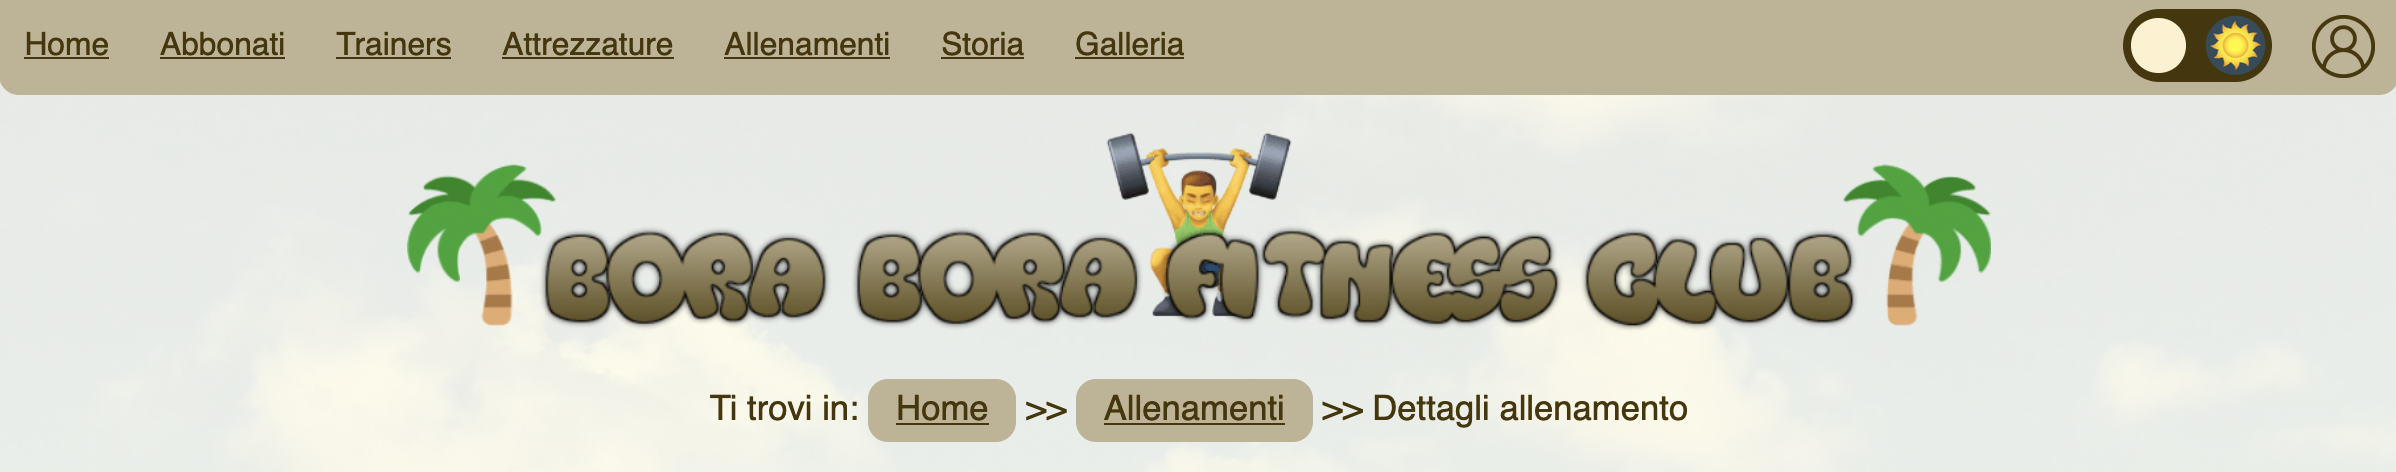
\includegraphics[scale=0.35]{immagini/header.png}
		\caption{Header}
	\end{figure}
	L'header è la prima sezione della pagina, fino al breadcrumb. È composta (nei file HTML) da tutto il contenuto compreso all'interno del tag <header>, tra cui:
	\begin{itemize}
		\item il menù di navigazione, sempre disponibile in cima alla pagina nella modalità desktop e nascosto sotto forma di burger menù nel formato tablet e mobile. Permette di accedere comodamente a tutte le pagine nel primo livello della gerarchia, oltre a cambiare lo schema dei colori tra le modalità light e dark. Il toggle per lo schema dei colori non fa parte, a livello di struttura, del menù di navigazione, ma è stato posto lì per semplificarne l'accesso tramite CSS;
		\item il titolo del sito, visualizzato sotto forma di immagine, ma reso accessibile con la tecnica di image replacement;
		\item il breadcrumb, che permette all'utente di ricordare in quale pagina si trova e il percorso effettuato per raggiungerla, fornendo anche i link per tornare alle pagine precedentemente visitate.
	\end{itemize}
	Soltanto a livello visivo tramite CSS, ma non a livello di struttura, l'header contiene anche il titolo della pagina, che ne riassume il contenuto. Talvolta può essere corredato da un sottotitolo, che specifica più nel dettaglio i contenuti trattati nella pagina, per aiutare l'utente a rispondere più velocemente e accuratamente alla domanda “Di cosa si tratta?” e incentivarlo a proseguire nella lettura.
	
	\subsubsection{Contenuto} \label{contenuto}
	Di seguito vengono elencate le pagine che compongono il sito:
	\begin{itemize}
		\item \textbf{Home:} è la prima pagina che viene visualizzata quando un utente visita il sito e ha lo scopo di far capire all'utente cosa può fare all'interno del sito. La pagina mostra le informazioni più importanti sulla palestra (come raggiungerci, orari di apertura, ecc.) e presenta una sezione che ha lo scopo di convincere l'utente ad iscriversi ad essa. È inoltre presente un link che porta alle proprie schede di allenamento il quale è una delle prime informazioni che vengono visualizzate nel layout mobile, questo per facilitare la navigazione agli utenti che vogliono consultare la propria scheda di allenamento dal telefono mentre sono in palestra.
		\item \textbf{Abbonati:} in questa pagina vengono illustrati i diversi tipi di abbonamento disponibili ed ulteriori dettagli sull'iscrizione, da questa pagina è inoltre possibile accedere alla pagina di acquisto abbonamento.
		\item \textbf{Acquista abbonamento:} questa pagina accessibile solo agli utenti autenticati permette di scegliere una tipologia di abbonamento ed acquistarla, una volta effettuato l'acquisto l'utente verrà reindirizzato alla sua area personale.
		\item \textbf{Trainers:} questa pagina illustra i personal trainer che lavorano all'interno della palestra, ad ogni personal trainer è associato nome, età, una citazione, una descrizione, i suoi corsi e le sue specializzazioni.
		\item \textbf{Attrezzature:} in questa pagina sono presenti le foto di tutte le macchine e gli attrezzi presenti nella palestra con la relativa descrizione.
		\item \textbf{Allenamenti:} all'interno di questa pagina è possibile consultare le informazioni principali delle schede di allenamento create dagli utenti. Ogni tipologia di utente può consultare un allenamento nel dettaglio tramite l'apposito link, mentre solo gli utenti autenticati possono seguire gli allenamenti di altri utenti, creare un nuovo allenamento, modificare ed eliminare i propri allenamenti. Gli admin possono modificare ed eliminare gli allenamenti di tutti gli utenti.
		\item \textbf{Crea allenamento:} questa pagina accessibile solo agli utenti autenticati presenta una form per la creazione di un allenamento, se la pagina è visualizzata da un admin offre anche la possibilità di assegnare l'allenamento ad un utente specifico.
		\item \textbf{Dettagli allenamento:} all'interno di questa pagina è possibile visualizzare nel dettaglio un allenamento con la possibilità di stamparlo. La pagina è visitabile anche da utenti non autenticati.
		\item \textbf{Modifica allenamento:} questa pagina permette di modificare un allenamento creato da un utente, aggiungendo o eliminando esercizi. È visitabile solamente dall'utente che ha creato quell'allenamento e da un admin.
		\item \textbf{Storia:} questa pagina illustra la storia della palestra a partire da quando è stata fondata fino al giorno d'oggi.
		\item \textbf{Galleria:} in questa pagina sono presenti le fotografie della palestra raggruppate in base alle diverse zone.
		\item \textbf{Area personale utente:} questa pagina accessibile solo agli utenti autenticati permette di visualizzare le proprie informazioni personali e modificarle, è inoltre possibile visualizzare le informazioni relative al proprio abbonamento e alle schede di allenamento create e seguite. È infine possibile effettuare il logout.
		\item \textbf{Area personale admin:} questa pagina accessibile solo agli admin offre le stesse funzionalità dell'area personale utente con l'aggiunta della gestione utenti (che non siano a loro volta degli amministratori) la quale permette di cercare o eliminare degli utenti o accedere alla loro area personale per visualizzare o modificare i dati relativi alle loro informazioni personali o relativi all'abbonamento e di visualizzare gli allenamenti seguiti e creati dall'utente.
		\item \textbf{Accesso:} questa pagina viene visualizzata quando un utente non registrato cerca di accedere ad una pagina che richiede l'autenticazione. Una volta effettuato l'accesso l'utente ora autenticato viene rimandato alla pagina che voleva inizialmente visualizzare.
		\item \textbf{Registrazione:} questa pagina è accessibile dalla pagina per effettuare il login. Permette all'utente non registrato di creare un proprio account per usufruire dei contenuti che richiedono l'autenticazione. Una volta effettuata la registrazione l'utente ha un proprio profilo, è automaticamente autenticato e viene rimandato alla pagina che inizialmente voleva visualizzare.
		\item \textbf{404:} questa pagina viene visualizzata solo nel caso in cui una risorsa non venga trovata a causa di un errore di ricerca da parte dell'utente. Sfrutta una emotional design consona al dominio del sito per fornire consigli utili a risolvere il problema e permette di essere reindirizzato verso le altre pagine del sito, in modo da poter cercare nuovamente il contenuto desiderato. Il file .htaccess gestisce l'errore 404 e rimanda a tale pagina.
		\item \textbf{500:} questa pagina viene visualizzata solo nel caso in cui una risorsa non venga trovata a causa di un errore interno del server. Sfrutta una emotional design consona al dominio del sito per fornire consigli utili a risolvere il problema e permette di essere reindirizzato verso le altre pagine del sito, in modo da poter cercare nuovamente il contenuto desiderato. Il file .htaccess gestisce l'errore 500 e rimanda a tale pagina.
	\end{itemize}
	
	\subsubsection{Footer}
	All'interno del footer compaiono elementi di generica utilità e informazioni importanti che non sono presenti nel resto del sito:
	\begin{itemize}
		\item contatti della palestra (nome, indirizzo, numero di telefono, email, social network quali Instagram e Facebook);
		\item dicitura per il copyright;
		\item icone per esibire la conformità agli standard W3C (HTML 5.0 e CSS);
		\item informazioni sui creatori del sito.
	\end{itemize}
	
	\subsubsection{Database}
	Il sito è stato pensato per offrire tutte le maggiori funzionalità che un utente di una palestra potrebbe aver bisogno. Ciò comprende la possibilità di gestire i propri dati e quelli relativi alle proprie attività di palestra, come accessi, abbonamenti e allenamenti. Ne consegue un database moderatamente composto in cui è stato posto particolare attenzione all'efficienza: essa risulta essere decomposta fino alla forma normale di Boyce-Codd, e di conseguenza anche tutte le forme normali precedenti. Non vi è quindi alcun problema di ridondanza dati, e ciò contribuisce ad alleviare il problema del peso di un database articolato e sperabilmente utilizzato da un gran numero di utenti in futuro.

	\paragraph{Schema concettuale}
	\begin{figure}[H]
		\centering
		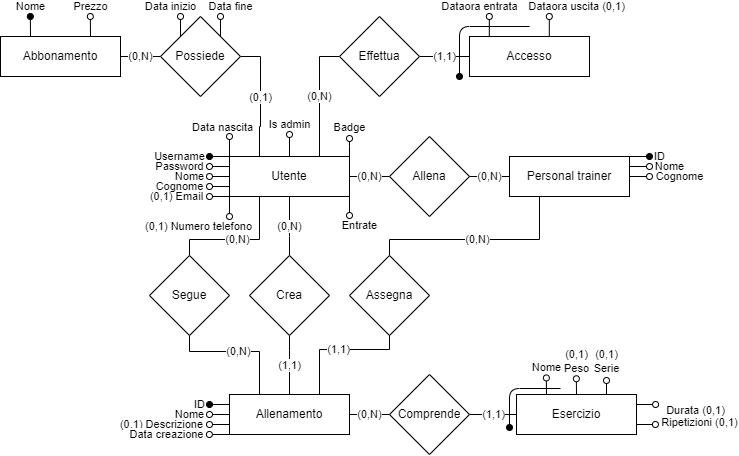
\includegraphics[scale=0.6]{immagini/schemaER.png}
		\caption{Schema concettuale del database.}
	\end{figure}

	Il sito non implementa le funzionalità per modificare le tabelle Abbonamento, Accesso e Personal trainer: queste vengono solo usate solo per visualizzarne i dati. Queste tabelle infatti vengono raramente modificate e in più il progetto originale del sito non prevede di implementare operazioni che richiedano di scrivere al loro interno. In particolare, in una situazione reale, la tabella Accesso sarebbe collegata ad un tornello all'ingresso della palestra, che aggiunge tuple alla tabella in base agli accessi dei clienti con i loro badge. Essendo che non disponiamo del tornello, questa tabella non cambia il suo contenuto.

	\paragraph{Schema logico}
	\texttt{{\bf abbonamento} (nome, prezzo)\\
		{\bf utente} (username, password, nome, cognome, email, data\_nascita, badge, entrate, numero\_telefono, nome\_abbonamento, data\_inizio, data\_fine, is\_admin)\\
		{\bf accesso} (username\_utente, dataora\_entrata, dataora\_uscita)\\
		{\bf personal\_trainer} (id, nome, cognome)\\
		{\bf utente\_personal\_trainer} (username\_utente, id\_personal\_trainer)\\
		{\bf allenamento} (id, nome, descrizione, username\_utente, data\_creazione, id\_personal\_trainer)\\
		{\bf utente\_allenamento} (username\_utente, id\_allenamento)\\
		{\bf esercizio} (id\_allenamento, nome, descrizione, peso, ripetizioni, serie, durata)\\
		utente.nome\_abbonamento → abbonamento.nome\\
		accesso.username\_utente → utente.username\\
		utente\_personal\_trainer.username\_utente → utente.username\\
		utente\_personal\_trainer.id\_personal\_trainer → personal\_trainer.id\\
		allenamento.username\_utente → utente.username\\
		allenamento.id\_personal\_trainer → personal\_trainer.id\\
		utente\_allenamento.username\_utente → utente.username\\
		utente\_allenamento.id\_allenamento → allenamento.id\\
		esercizio.id\_allenamento → allenamento.id
}

	\subsubsection{Ricerche probabili}
	Perché possa essere quanto più visibile in un motore di ricerca, il sito deve rispondere a delle query eseguite da utenti che non conoscono il sito e che stanno cercando una palestra, soprattutto a Bora Bora, che abbia degli spazi outdoor. Inoltre deve rispondere a ricerche relative ad allenamenti per la palestra e schede di allenamento, oltre a proposte di abbonamento in palestra. Di seguito vengono riportate le più probabili tra le ricerche possibili a cui dovrebbe rispondere il sito:
	\begin{itemize}
		\item palestra bora bora
		\item fitness bora bora
		\item allenarsi a bora bora
		\item palestra outdoor
		\item allenamento palestra
		\item allenamenti palestra
		\item schede allenamento
		\item scheda allenamento
		\item abbonamenti palestra
	\end{itemize}

	\section{Realizzazione}
	\subsection{Linguaggi}
	\begin{itemize}
		\item HTML5: abbiamo deciso di utilizzare lo standard HTML5 dato che secondo la nostra analisi dell'utenza, quasi tutti i visitatori del sito disporranno di dispositivi in grado di supportare questo standard. HTML5 ci permette di descrivere meglio la struttura della pagina con tag come article, header, footer, nav e altri. Inoltre ci è molto utile per alcune form dove al tag input vengono utilizzati i valori number, email, tel, date e time per l'attributo type. Tutte le pagine HTML che si possono visitare dal sito sono nella root del server;
		\item CSS3: è stato deciso di utilizzare lo standard css3 per facilitare la parte responsive del sito tramite l'utilizzo di flex e grid, inoltre i colori utilizzati dal sito sono salvati tramite variabili per facilitare la modifica e l'utilizzo della dark-mode, ci siamo assicurati che in ogni caso il sito sia usabile anche da browser vecchi che non supportano variabili, flex o grid;
		\item JavaScript: utilizzato per la validazione delle form lato client, l'implementazione della dark-mode e altre piccole features volte a migliorare la user experience. Non è stata utilizzata alcuna libreria esterna. Tutte le funzionalità sono state inserite in un unico file in una apposita cartella;
		\item PHP: utilizzato per la realizzazione di pagine web dinamiche, per le interazioni col database e la validazione delle form lato server. Tutte le pagine PHP che si possono visitare dal sito sono nella root del server e usano pagine HTML e PHP in apposite cartelle rispettivamente per inserire dati dinamicamente e come funzioni ausiliarie;
		\item SQL: usato MySQL (MariaDB). Utilizzato per la creazione del database e per effettuare le query di ricerca per generare pagine dinamiche in PHP. Vengono caricate le query per la creazione e un primo popolamento del database in un'apposita cartella.

	\end{itemize}

	\subsection{Strumenti}
	\begin{itemize}
		\item GitHub: strumento fondamentale per la collaborazione asincrona allo sviluppo del progetto;
		\item Strumenti per sviluppatore Chrome
		\item Strumenti per sviluppatore Firefox
		\item Xampp: software utilizzato per creare un web hosting locale che ci ha permesso di testare il sito anche da smartphone e tablet;
		\item \href{https://webaim.org/resources/contrastchecker/}{https://webaim.org/resources/contrastchecker/} strumento utilizzato per la verifica del contrasto tra i colori presenti nel nostro sito;
		\item \href{https://tools.pingdom.com/}{https://tools.pingdom.com/} strumento utilizzato per calcorare il peso delle pagine del sito.
		\item \href{https://validator.w3.org}{https://validator.w3.org} per la validazione del codice HTML5
		\item \href{https://jigsaw.w3.org/css-validator/}{https://jigsaw.w3.org/css-validator/} per la validazione del codice CSS
	\end{itemize}

	\section{Accessibilità}
	Per mantenere un alto livello di accessibilità ci siamo attenuti allo standard WCAG 2.0 (\href{https://www.w3.org/Translations/WCAG20-it/}{https://www.w3.org/Translations/WCAG20-it/})

	\subsection{Separazione tra comportamento, struttura e presentazione}
	Per migliorare l'accessibilità per gli utenti con differenti disabilità e per un miglior posizionamento nei motori di ricerca, abbiamo mantenuto una netta separazione tra comportamento, struttura e presentazione.
	Per quanto riguarda la struttura abbiamo utilizzato documenti HTML5, i quali sono stati stilizzati utilizzando documenti CSS esterni. Per il comportamento invece è stato utilizzato un documento Javascript esterno.
	Nel codice HTML non abbiamo inserito attributi relativi ad eventi Javascript in modo tale da separare completamente struttura da comportamento. Proprio per questo motivo è il codice Javascript a specificare gli eventi per ogni elemento HTML.
	Tutto il codice è stato scritto seguendo le raccomandazioni W3C, evitando l'utilizzo di tag e attributi deprecati, accertando la validità tramite l'utilizzo dei validatori.


	\subsection{WAI-ARIA}
	Per garantire l'accessibilità abbiamo deciso di utilizzare la specifica WAI-ARIA prodotta da W3C, che definisce un insieme di attributi HTML addizionali che possono essere applicati ai vari elementi per fornire maggior valore semantico e aumentare l'accessibilità. In particolare abbiamo utilizzato gli aria-label in quelle situazioni in cui non era presente testo, come per esempio il simbolo nel menù contenente il link per andare nell'area personale e nel footer nelle varie immagini utilizzate per le informazioni di contatto. Abbiamo inoltre utilizzato l'attributo aria-label anche sul breadcrumb per indicare che il contenuto di quel tag <nav> indica la posizione dell'utente all'interno del sito. Sempre riguardo alla navigazione, in ogni pagina abbiamo predisposto un link nascosto agli utenti ma visibile agli screen reader per saltare la lettura delle varie voci del menù e andare direttamente al contenuto della pagina. Per migliorare ulteriormente la navigazione, abbiamo predisposto un pulsante torna su che permette di tornare all'inizio della pagina. Per rendere accessibile la pagina dove è presente l'animazione del processo di pagamento, abbiamo inserito a inizio pagina, prima del menù, un <p> invisibile ma leggibile dagli screen reader per avvisare l'utente che utilizza una tecnologia assistiva della processazione del pagamento. Questo era necessario in quanto siccome la pagina effettua un redirect in pochi secondi, questa tipologia di utenti deve essere avvertita velocemente, evitando di rileggere il menù prima di venire a conoscenza di tale messaggio. Per quanto riguarda i form, ovunque ci fossero dei tag <p> predisposti per visualizzare degli errori negli input, abbiamo aggiunto l'attributo role=”alert” per attirare l'attenzione dell'utente che utilizza una tecnologia assistiva. Inoltre, per indicare quali campi fossero obbligatori abbiamo utilizzato l'attributo required di HTML5 che offre qualche funzionalità in più rispetto aria-required in quanto, oltre a garantire l'accessibilità, previene l'invio del form qualora il campo di input sia vuoto, senza l'utilizzo di Javascript.

	\subsection{Colori}
	I colori principali del sito sono color sabbia per gli sfondi dei <div>, marrone scuro per il testo e altri colori sempre sulle tonalità del marrone per vari elementi delle pagine. Come background abbiamo scelto un'immagine delle spiagge di Bora Bora. All'interno delle nostre pagine siamo stati attenti a non veicolare le informazioni tramite il solo utilizzo del colore, infatti per esempio tutti i link sono segnalati tramite sottolineatura oltre al colore di sfondo. Di seguito vengono riportati i risultati dei test effettuati su tutti i contrasti tra il colore del testo e il colore di sfondo presenti nel sito. In generale tutti i rapporti superano il test WCAG AA (minimo rapporto di 4.5:1 per testo normale e 3:1 per testo grande) ma la maggior parte sono WCAG AAA (minimo rapporto di 7:1 per testo normale e 4.5:1 per testo grande). Essendo i <div> semitrasparenti, nei contrasti dei colori che li utilizzano come colore di background abbiamo considerato la tonalità di colore più svantaggiosa per il contrasto.


	\subsubsection{Test colori light mode}
	\begin{figure}[H]
		\centering
		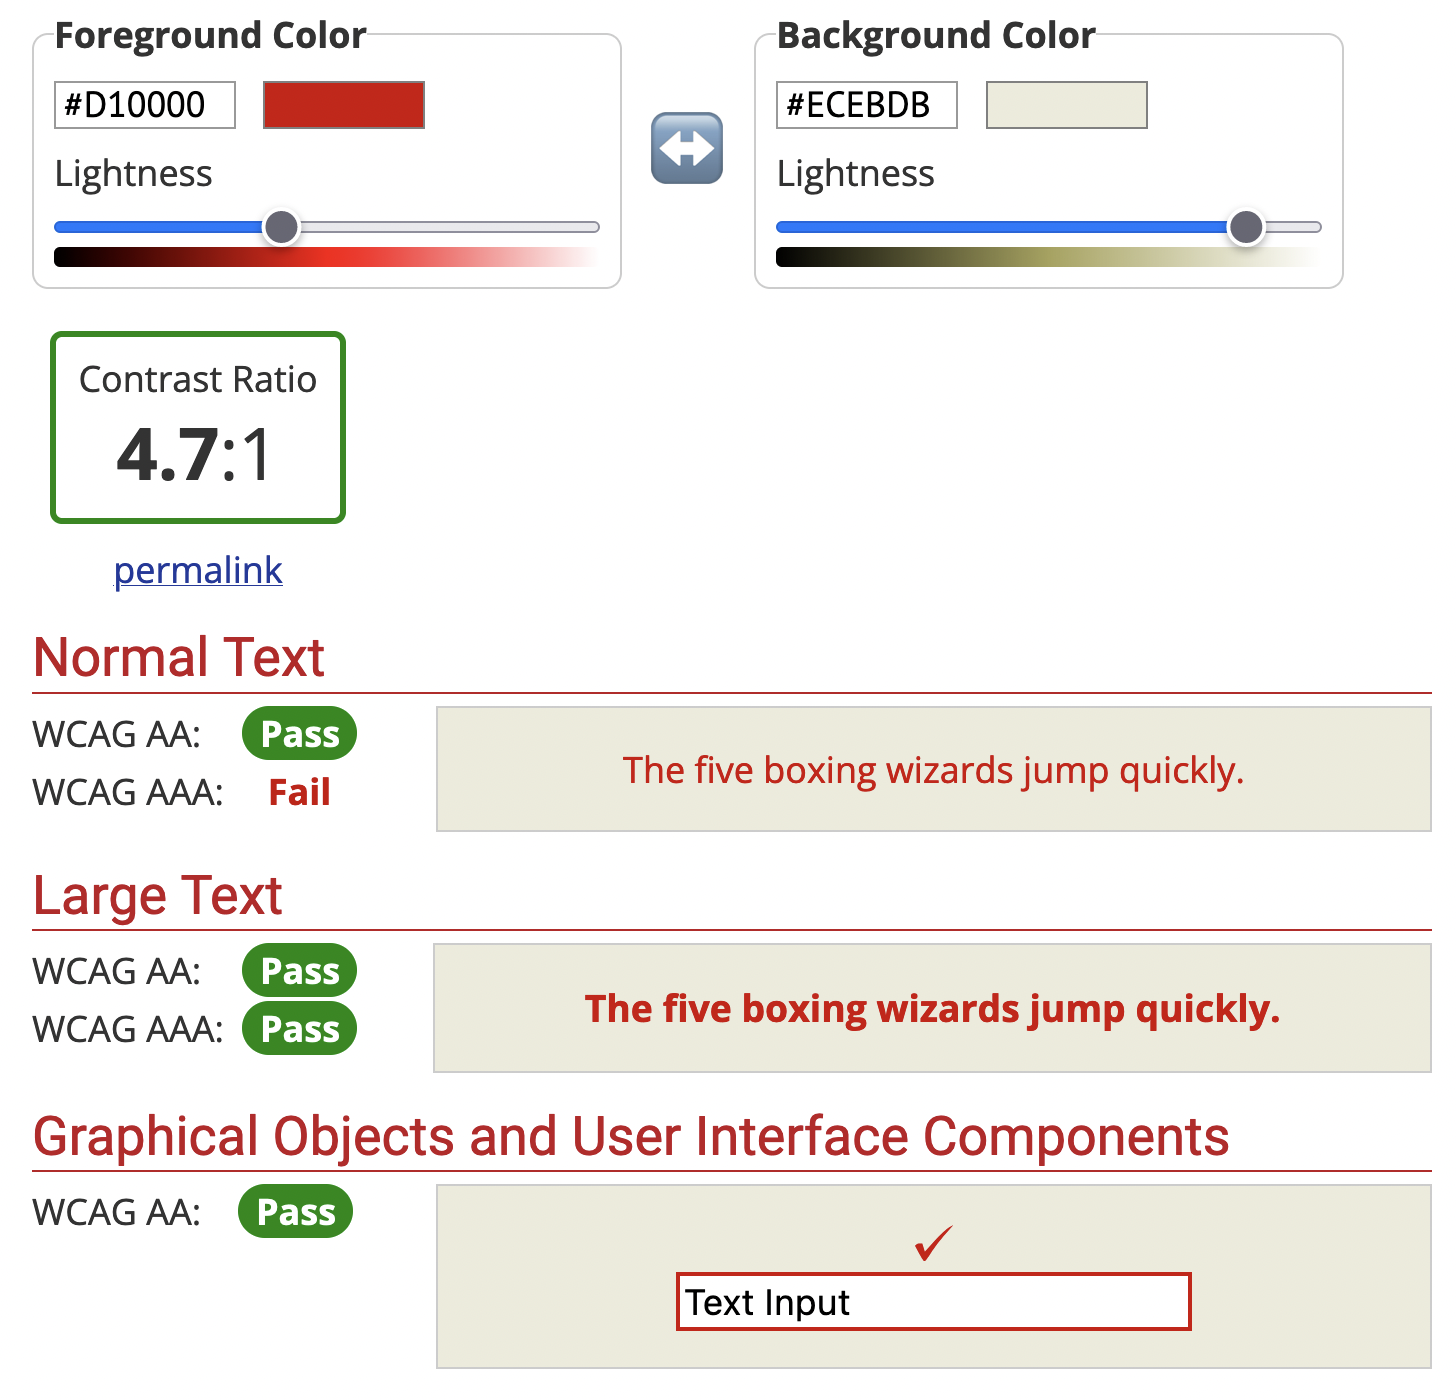
\includegraphics[scale=0.3]{immagini/controllo-colori/light-mode/errore_sfondo-div.png}
		\caption{Contrasto tra colore degli errori e sfondo del div.}
	\end{figure}

	\begin{figure}[H]
		\centering
		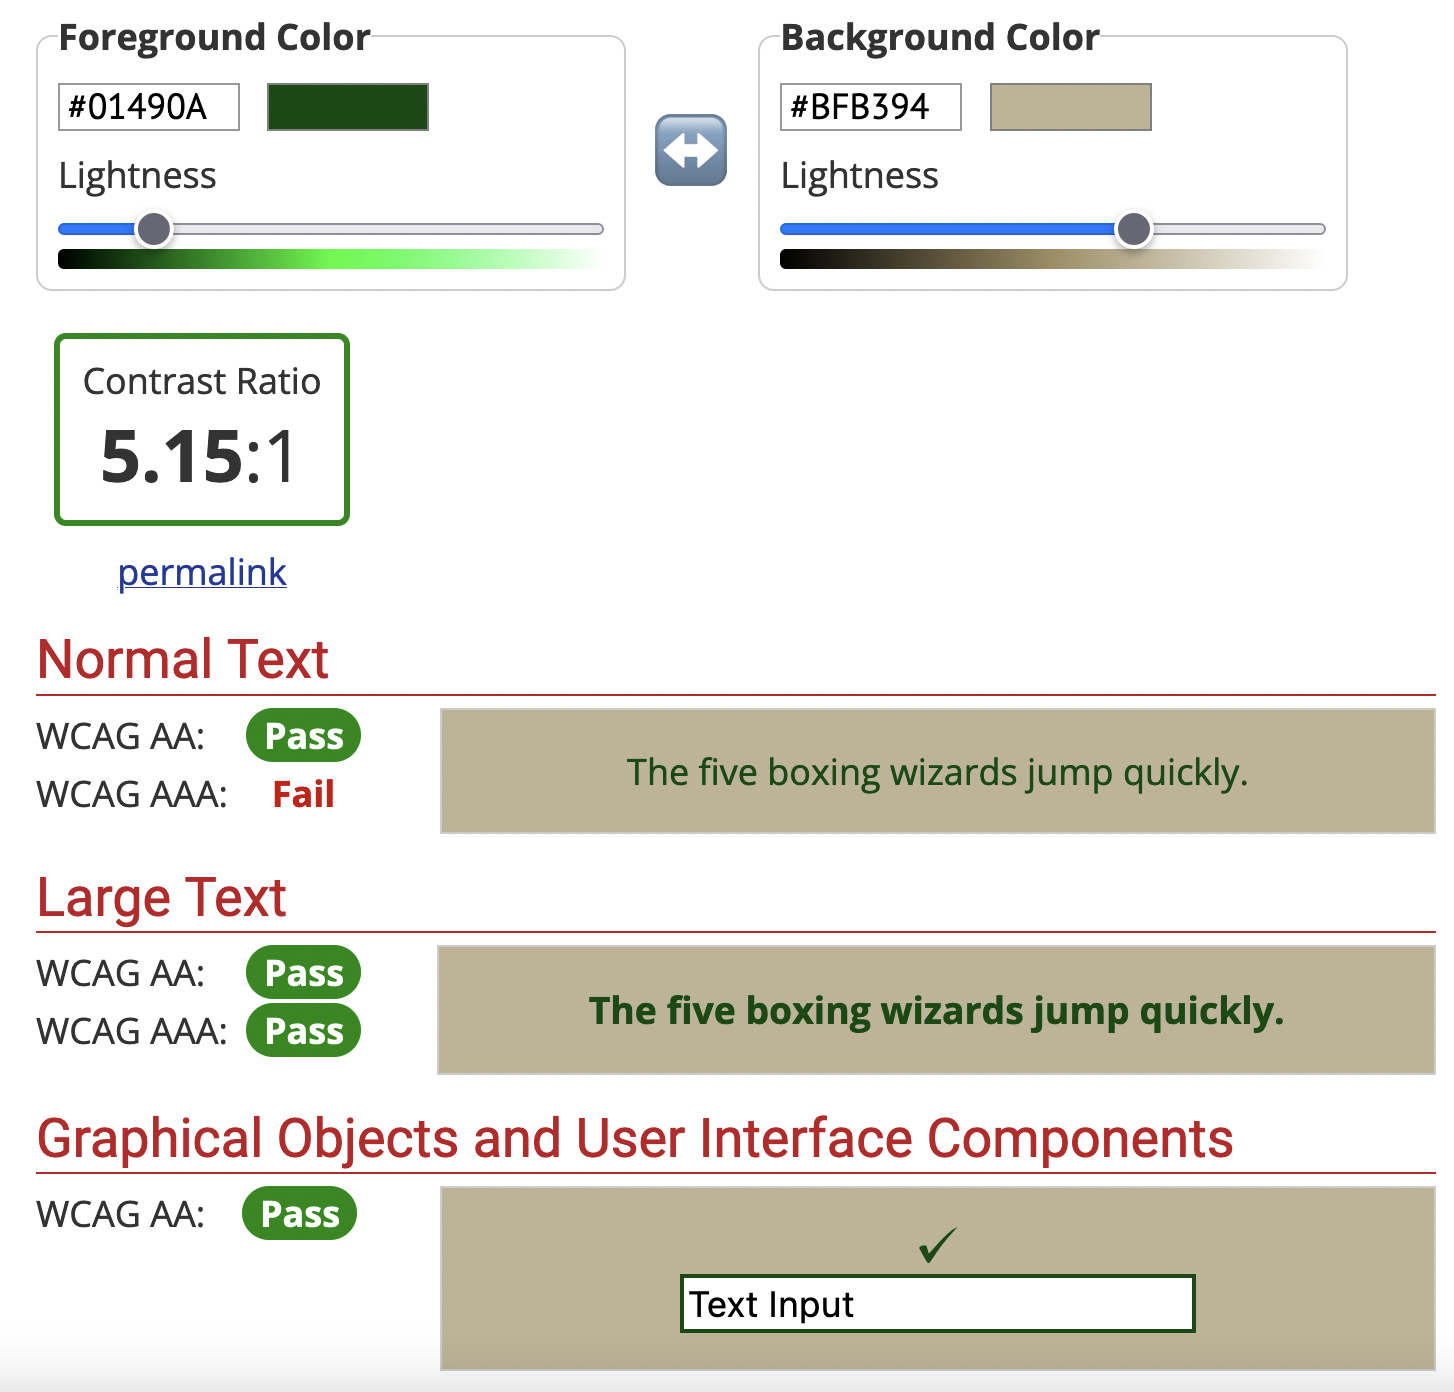
\includegraphics[scale=0.3]{immagini/controllo-colori/light-mode/link-da-visitare_background-menu.png}
		\caption{Contrasto tra colore dei link ancora da visitare e sfondo del menu in modalità desktop.}
	\end{figure}

	\begin{figure}[H]
		\centering
		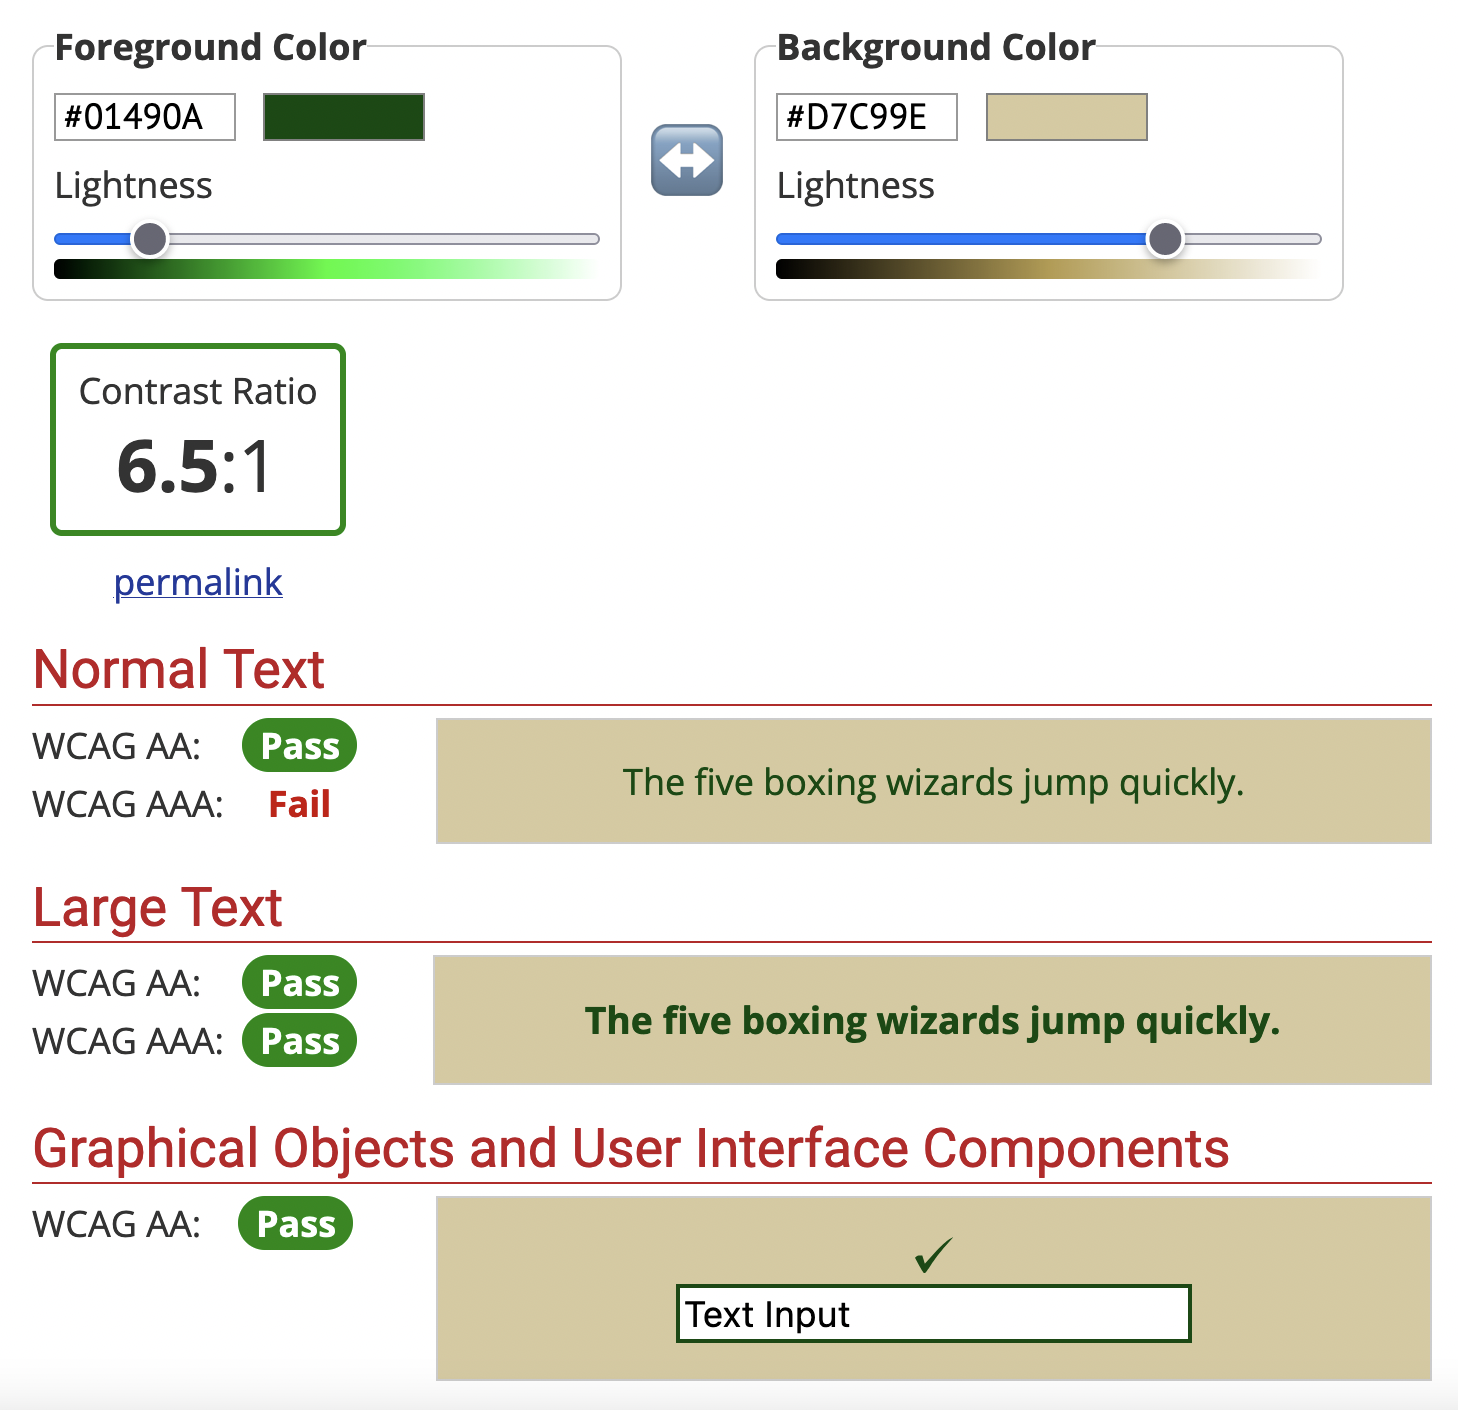
\includegraphics[scale=0.3]{immagini/controllo-colori/light-mode/link-da-visitare_sfondo-article-p.png}
		\caption{Contrasto tra colore dei link ancora da visitare e colore di sfondo dei link.}
	\end{figure}

	\begin{figure}[H]
		\centering
		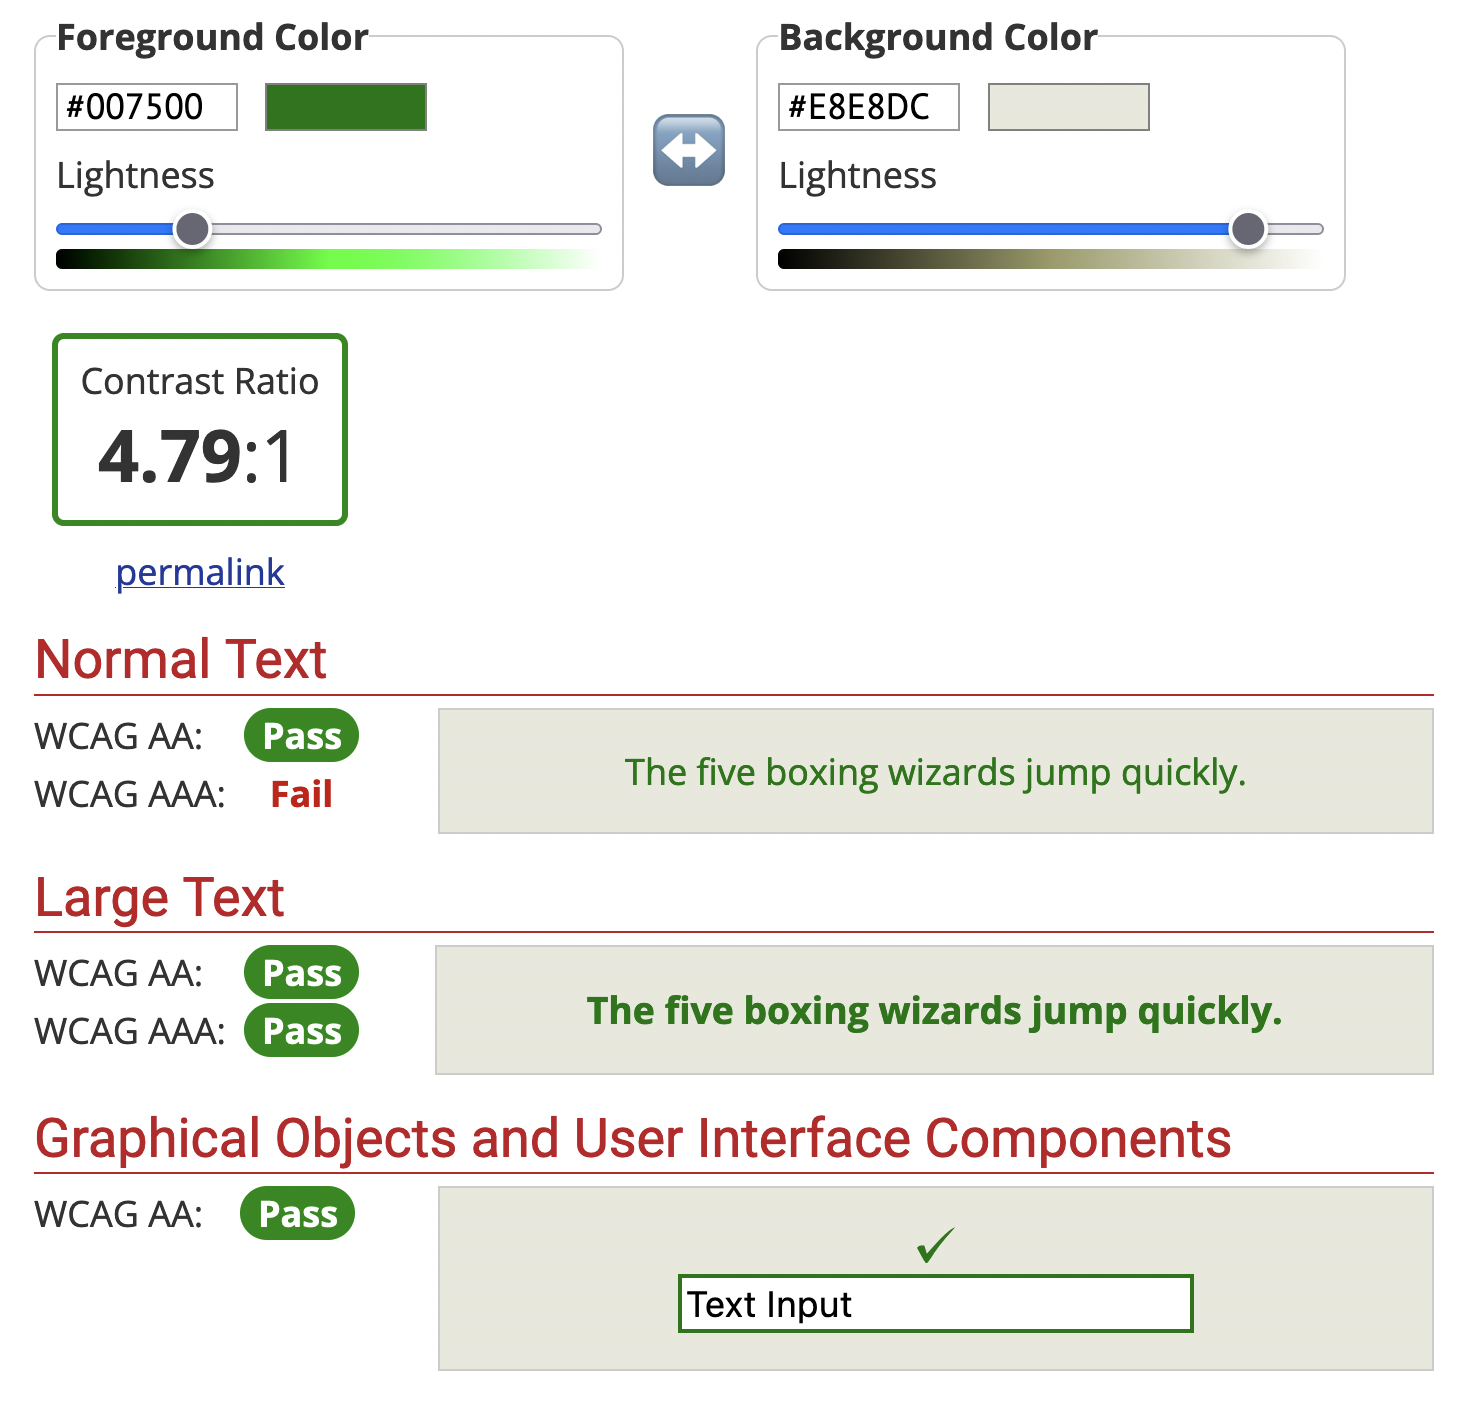
\includegraphics[scale=0.3]{immagini/controllo-colori/light-mode/successo_sfondo-div.png}
		\caption{Contrasto tra colore dei messaggi di successo e sfondo del div.}
	\end{figure}

	\begin{figure}[H]
		\centering
		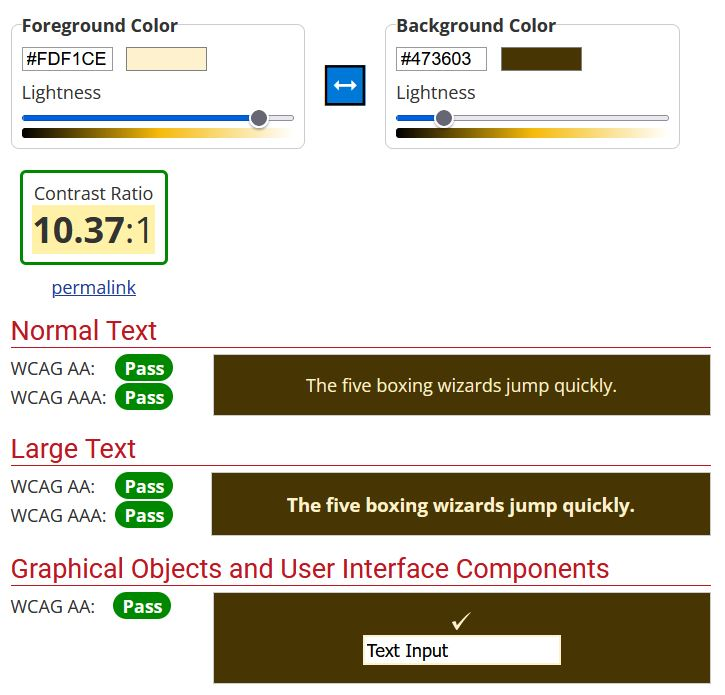
\includegraphics[scale=0.35]{immagini/controllo-colori/light-mode/testo-contrasto-sfondi_testo-principale.JPG}
		\caption{Contrasto tra colore del testo di \#currentLink nel menù e il suo sfondo in modalità desktop.}
	\end{figure}

	\begin{figure}[H]
		\centering
		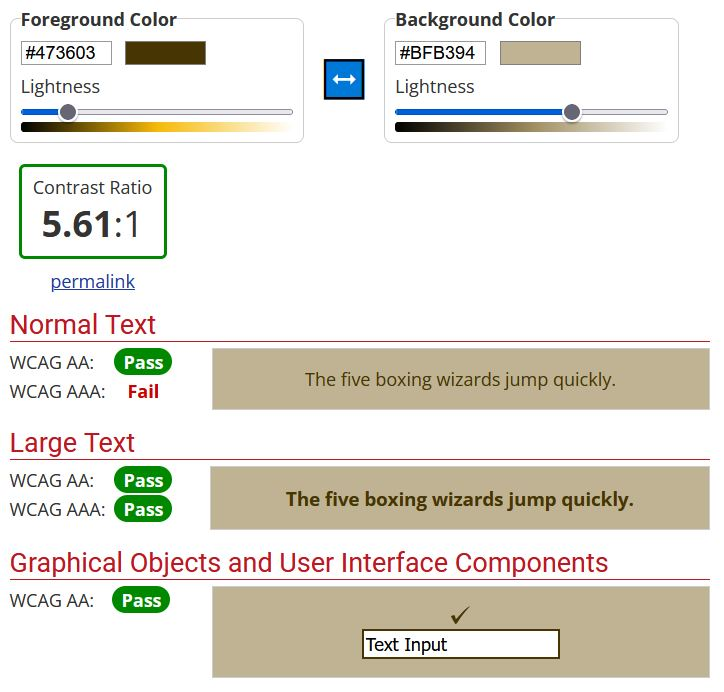
\includegraphics[scale=0.35]{immagini/controllo-colori/light-mode/testo-principale_background-menu.JPG}
		\caption{Contrasto tra colore dei link del menù e il loro sfondo in modalità desktop.}
	\end{figure}

	\begin{figure}[H]
		\centering
		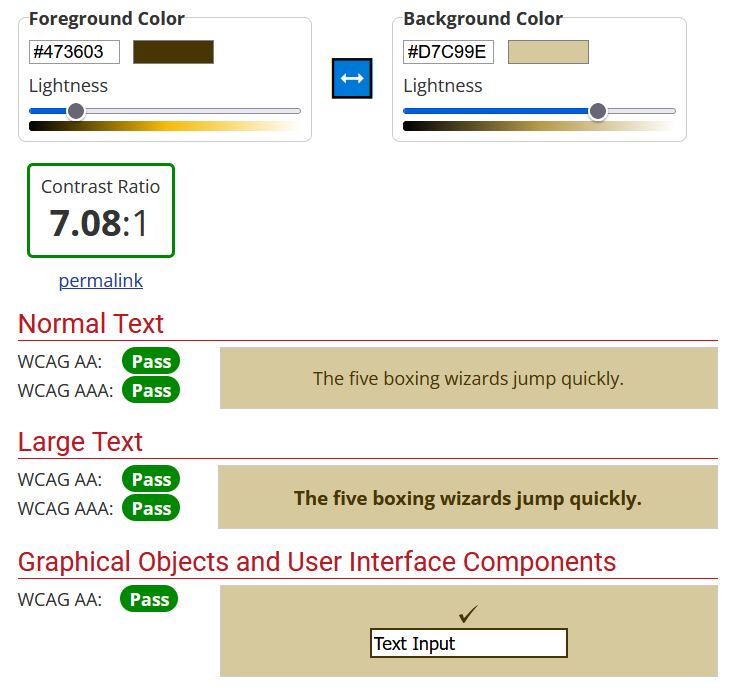
\includegraphics[scale=0.35]{immagini/controllo-colori/light-mode/testo-principale_sfondo-article-p.JPG}
		\caption{Contrasto tra colore del testo principale e sfondo delle schede degli allenamenti.}
	\end{figure}

	\begin{figure}[H]
		\centering
		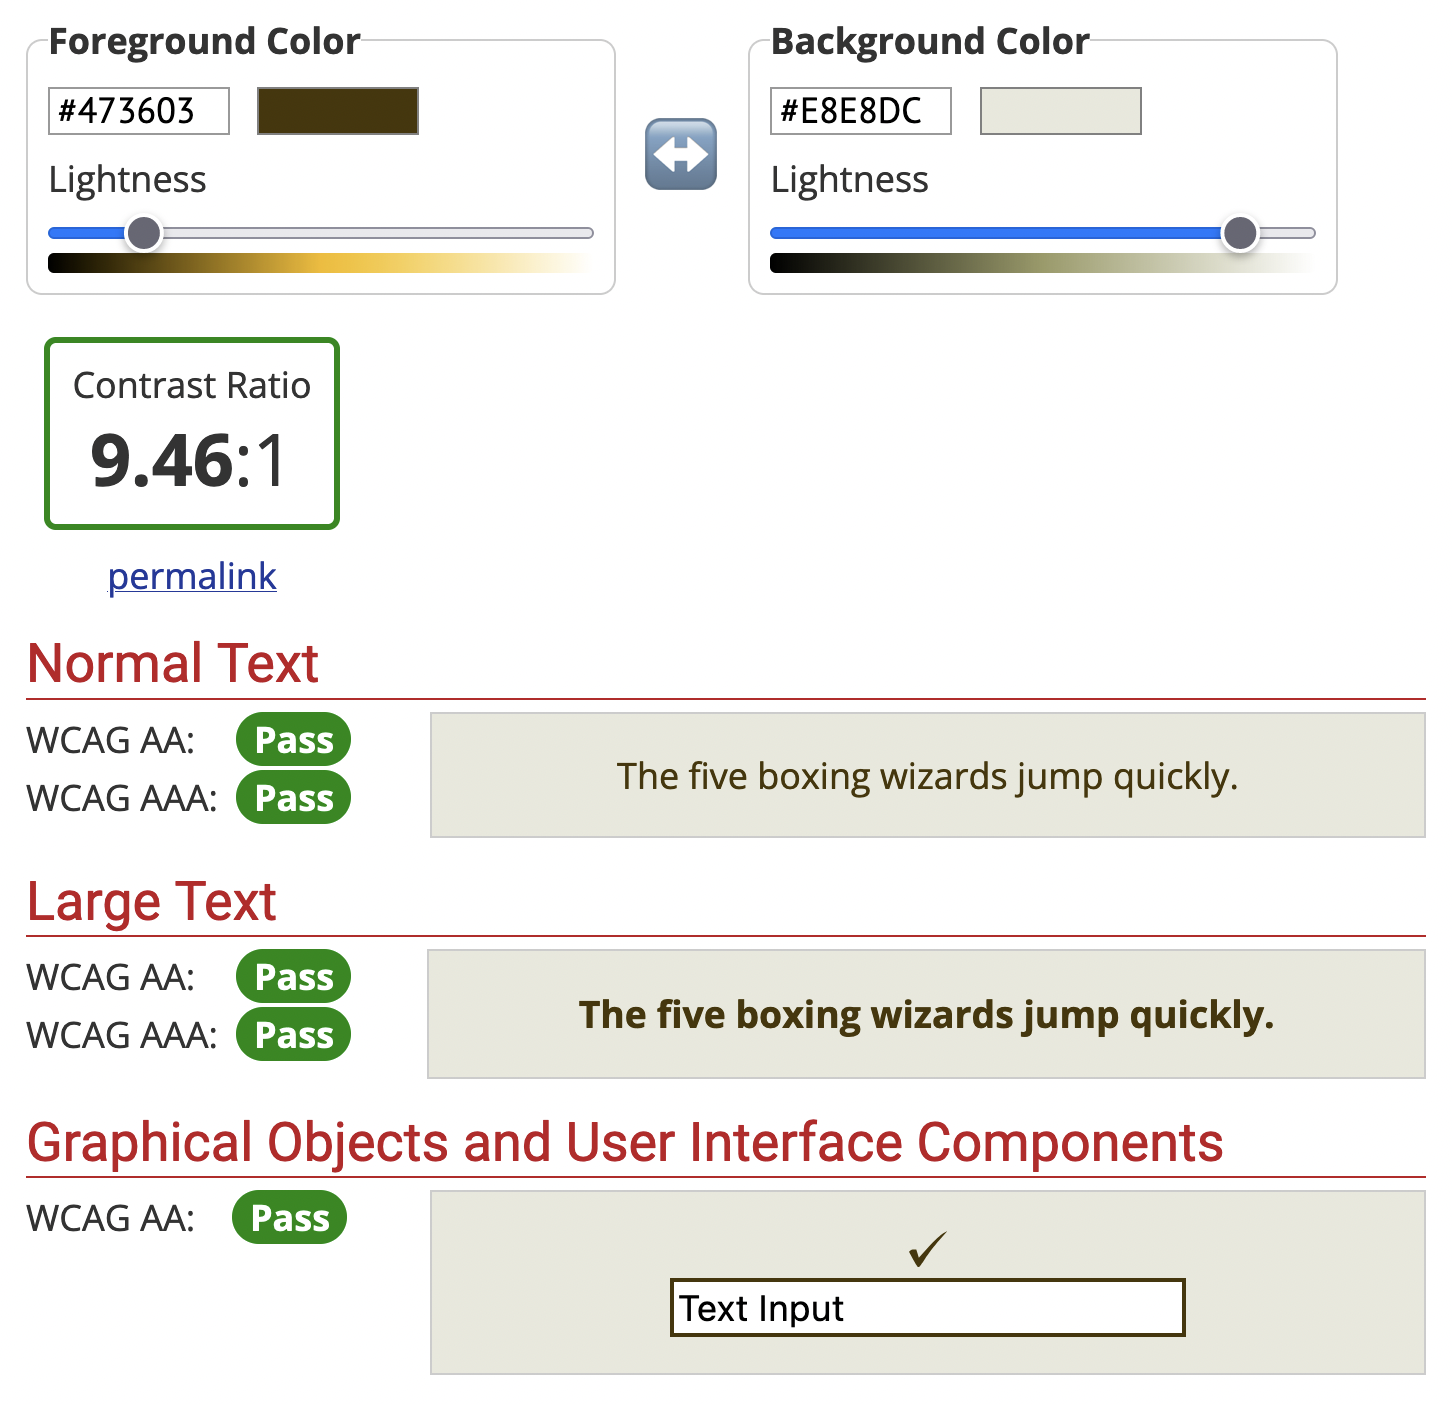
\includegraphics[scale=0.3]{immagini/controllo-colori/light-mode/testo-principale_sfondo-div.png}
		\caption{Contrasto tra colore del testo principale e sfondo dei div.}
	\end{figure}

	\subsubsection{Test colori dark mode}
	\begin{figure}[H]
		\centering
		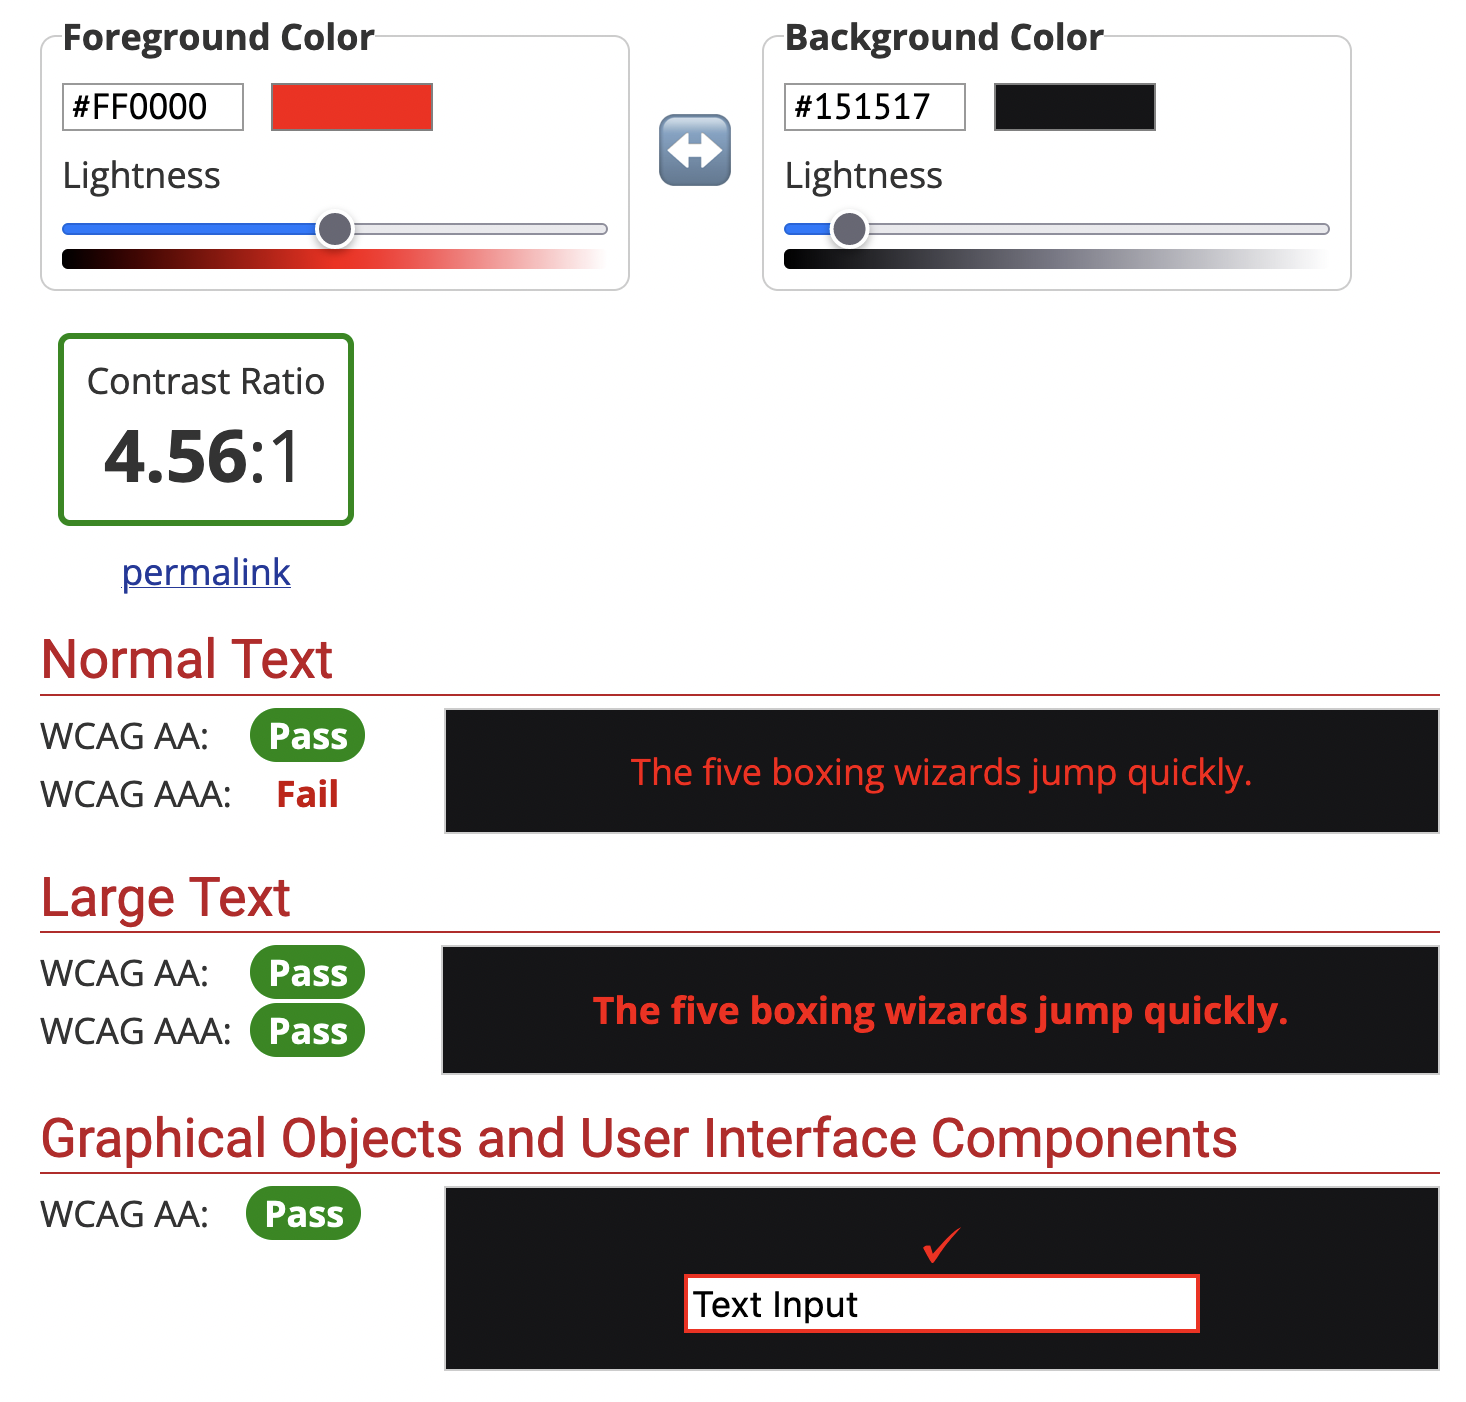
\includegraphics[scale=0.3]{immagini/controllo-colori/dark-mode/errore_sfondo-div.png}
		\caption{Contrasto tra colore degli errori e sfondo del div.}
	\end{figure}

	\begin{figure}[H]
		\centering
		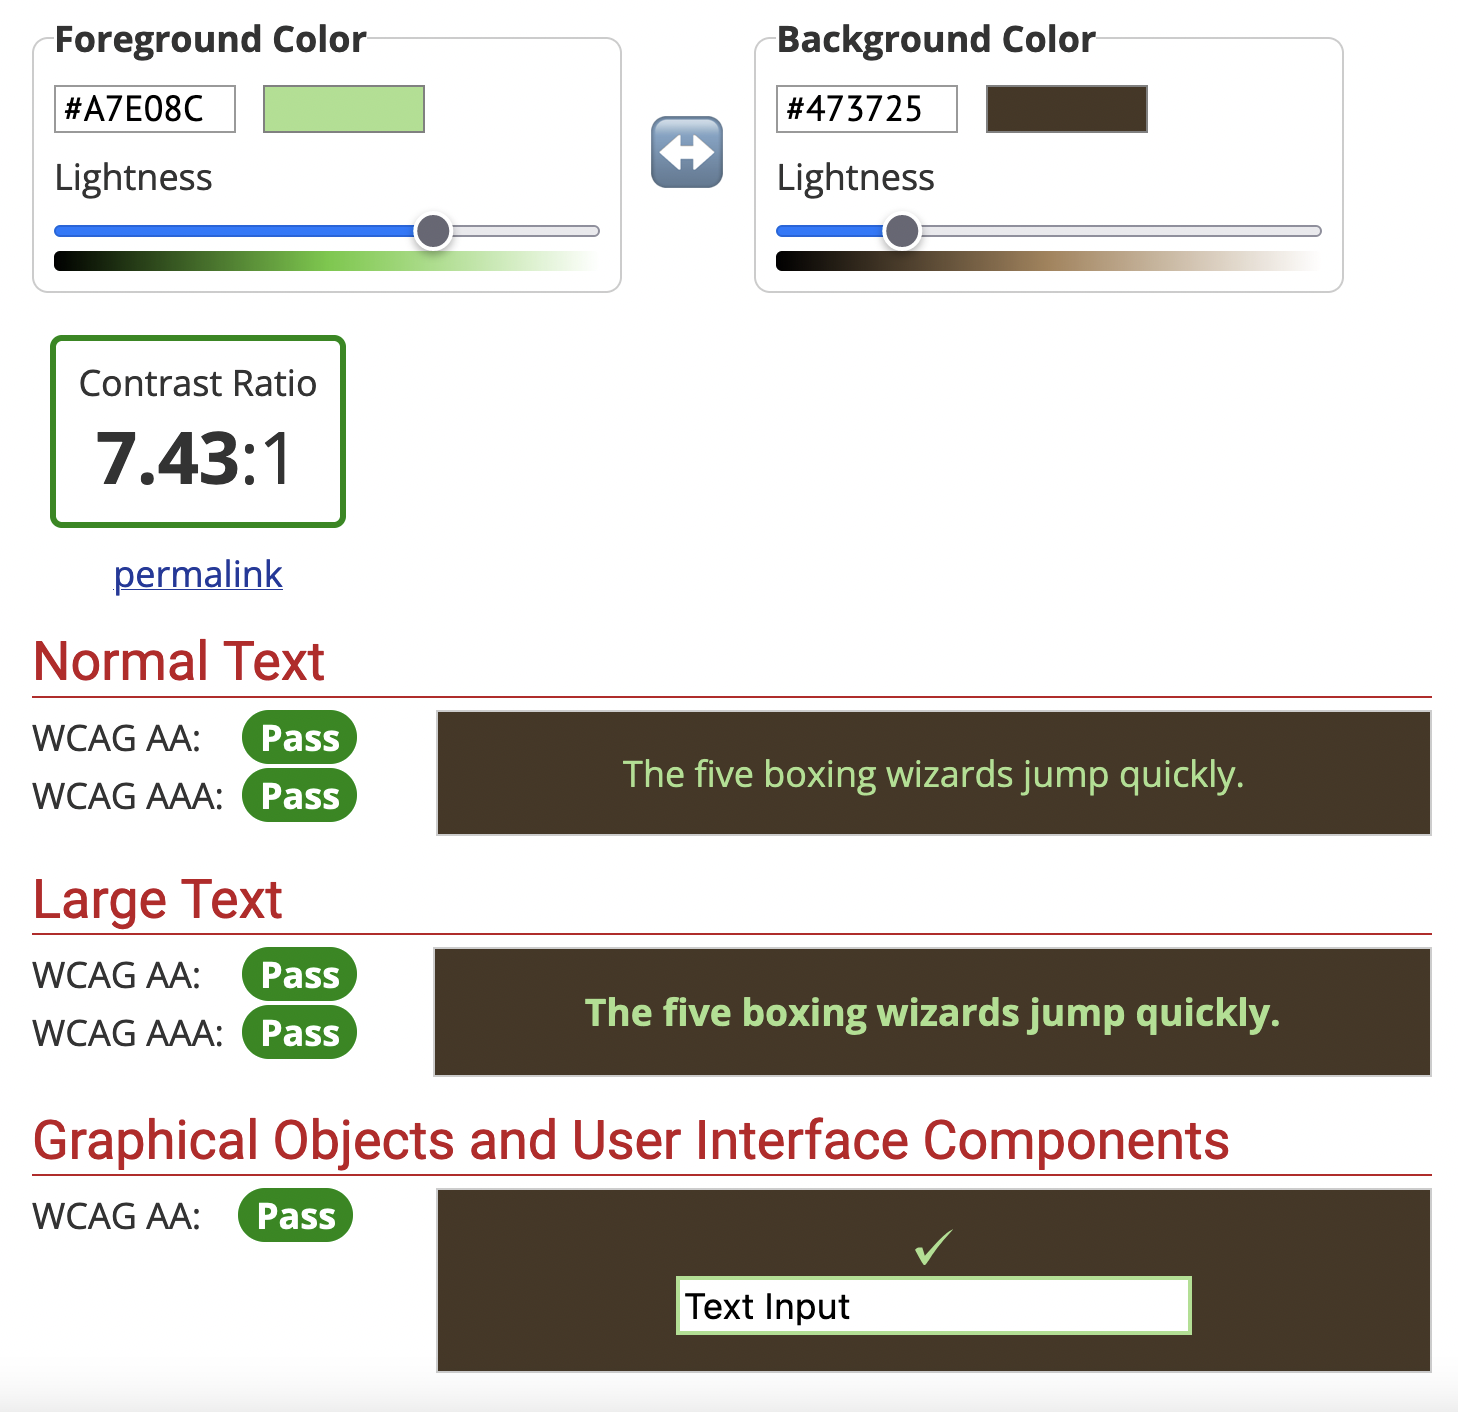
\includegraphics[scale=0.3]{immagini/controllo-colori/dark-mode/link-da-visitare_background-menu.png}
		\caption{Contrasto tra colore dei link ancora da visitare e sfondo del menu in modalità desktop.}
	\end{figure}

	\begin{figure}[H]
		\centering
		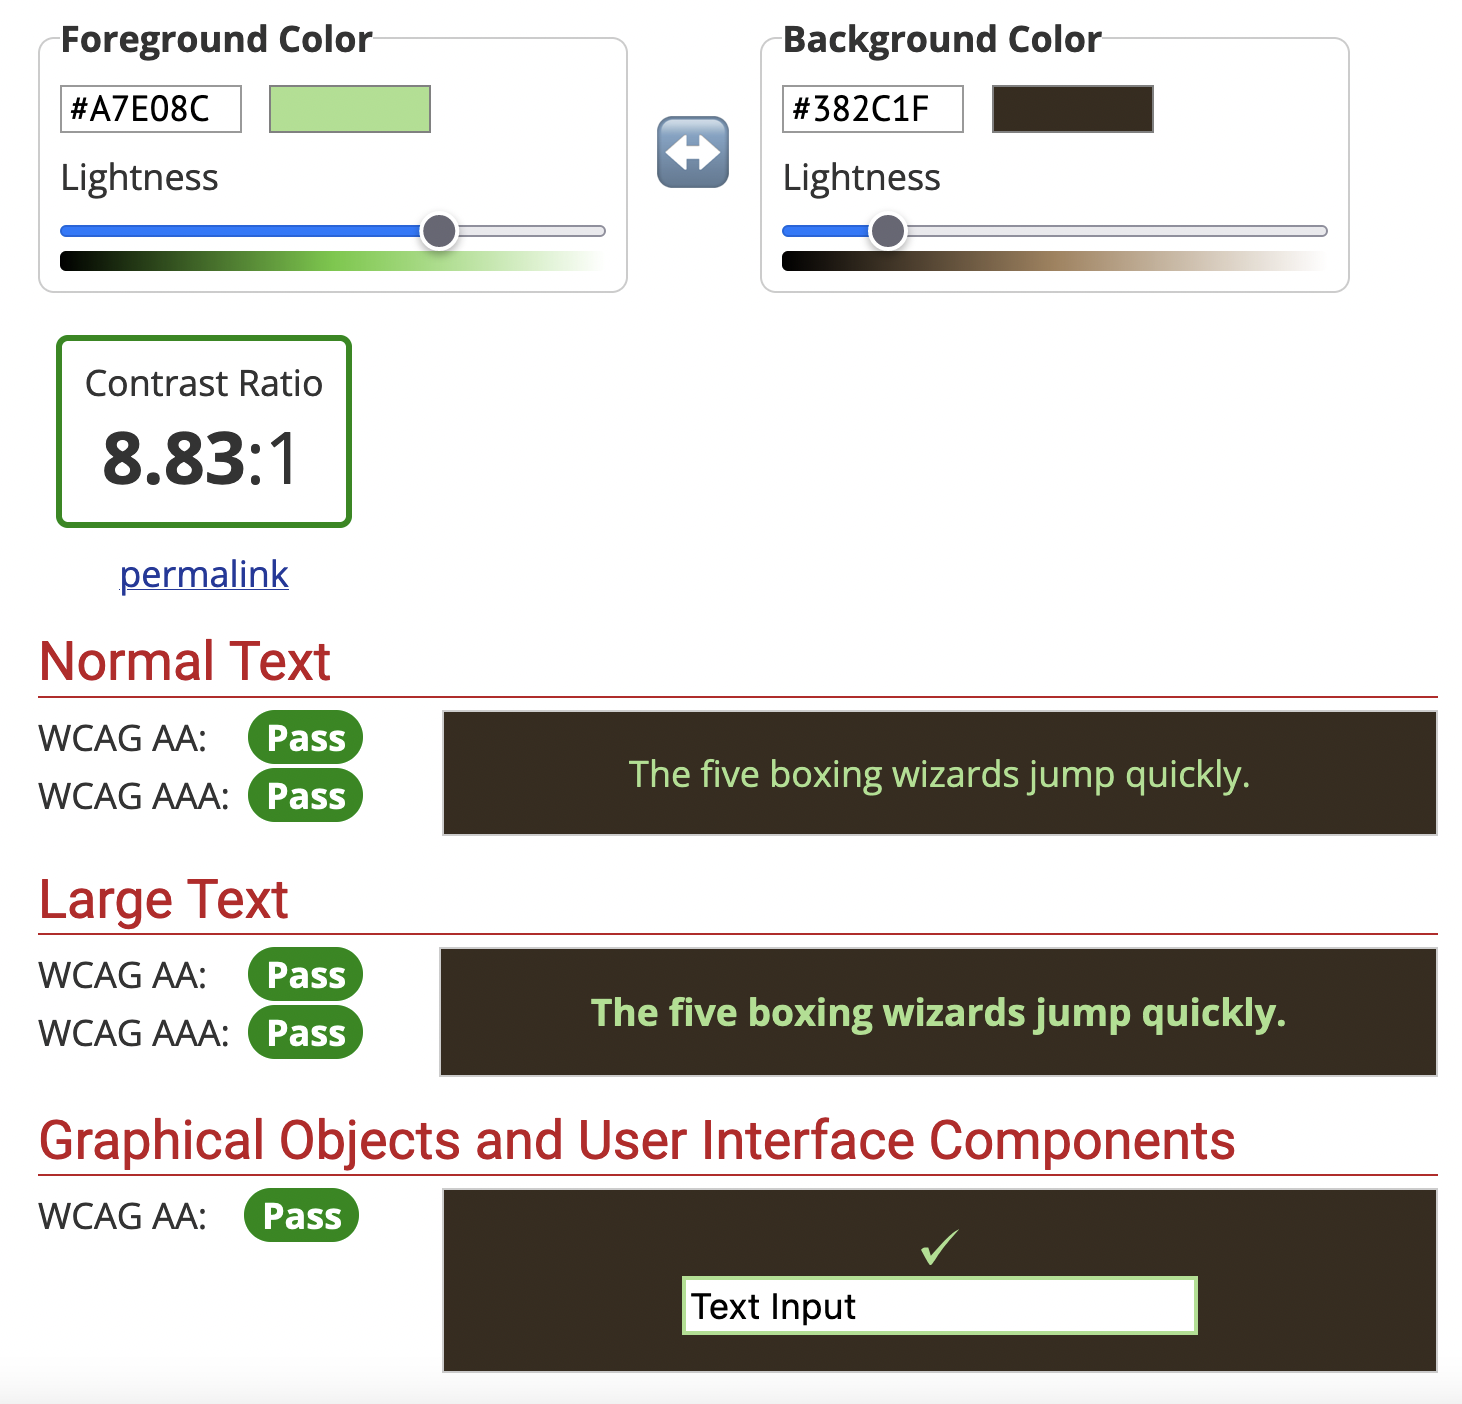
\includegraphics[scale=0.3]{immagini/controllo-colori/dark-mode/link-da-visitare_sfondo-article-p.png}
		\caption{Contrasto tra colore dei link ancora da visitare e colore di sfondo dei link.}
	\end{figure}

	\begin{figure}[H]
		\centering
		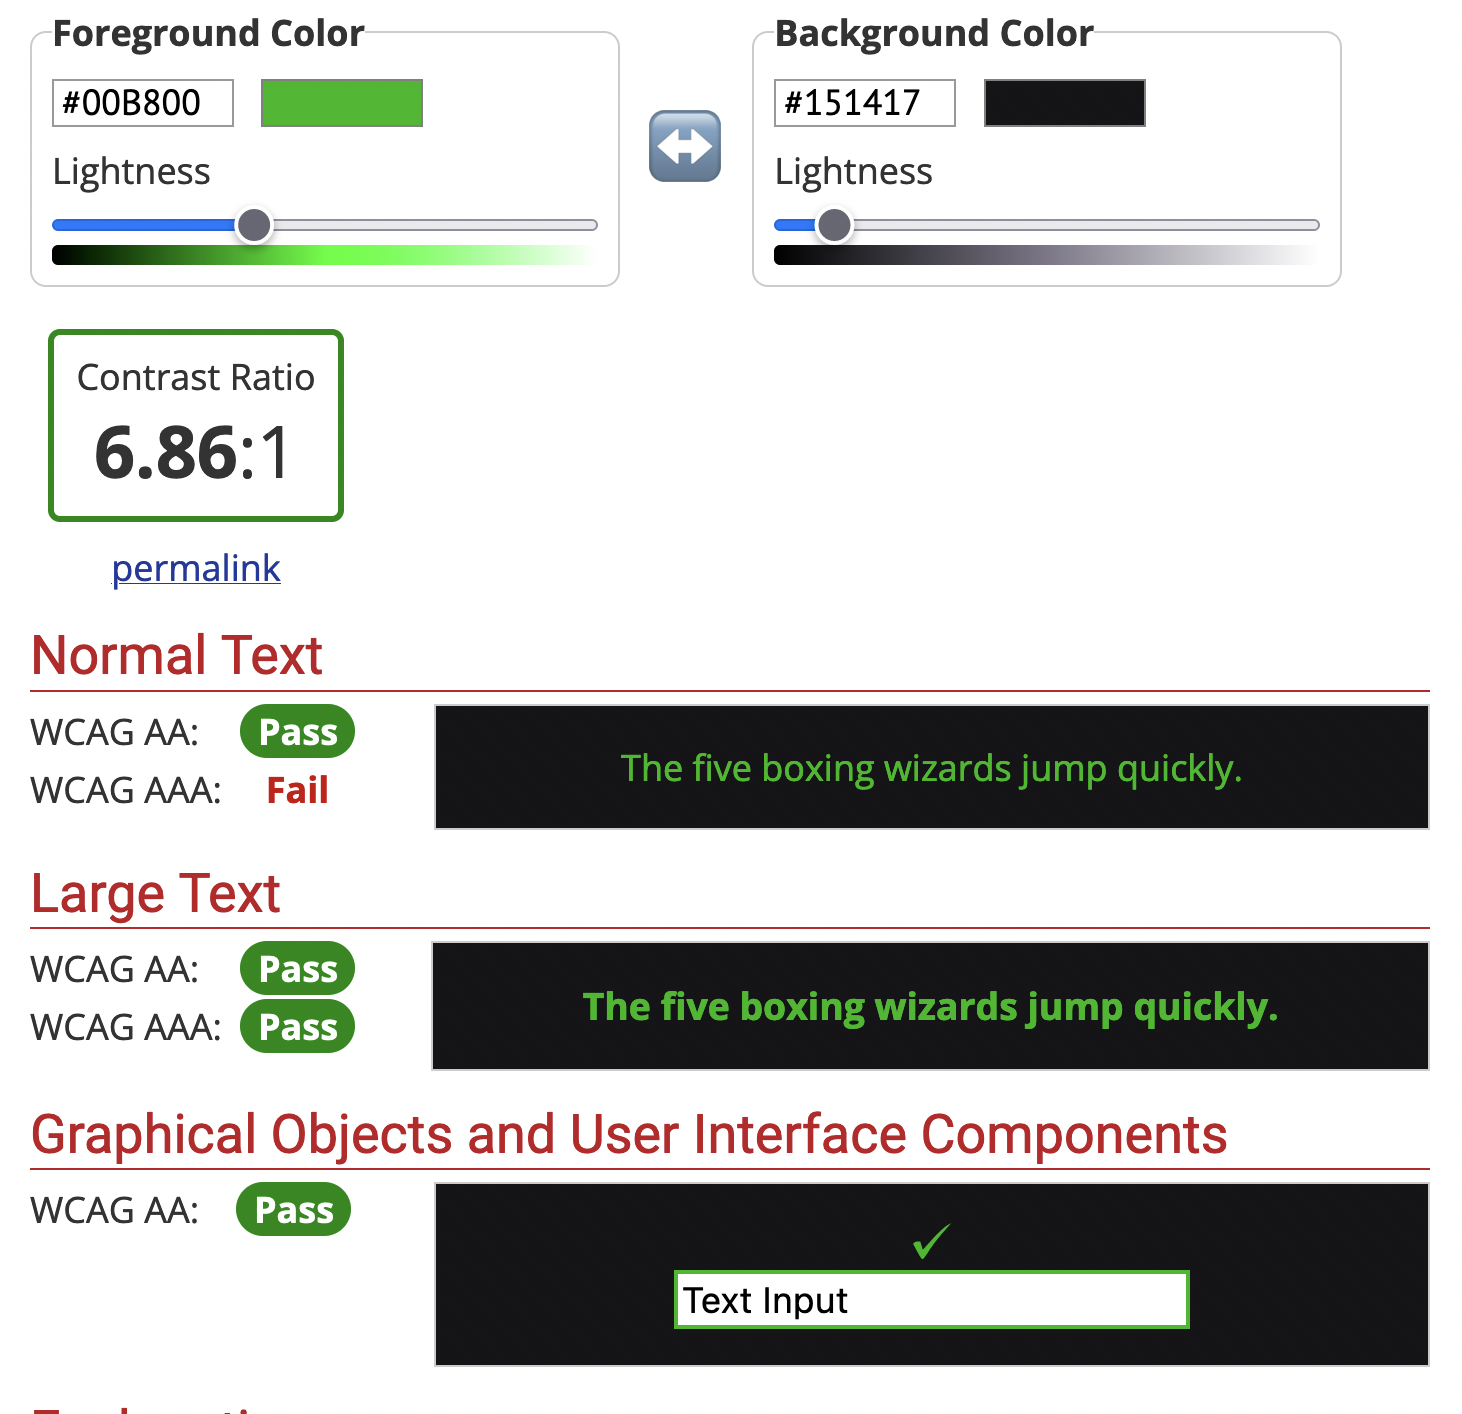
\includegraphics[scale=0.3]{immagini/controllo-colori/dark-mode/successo_sfondo-div.png}
		\caption{Contrasto tra colore dei messaggi di successo e sfondo del div.}
	\end{figure}

	\begin{figure}[H]
		\centering
		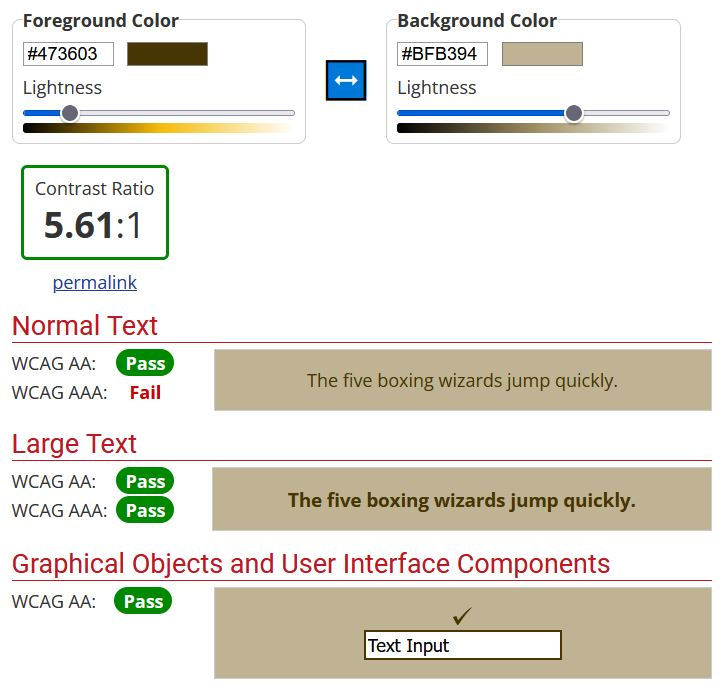
\includegraphics[scale=0.35]{immagini/controllo-colori/dark-mode/testo-contrasto-sfondi_testo-principale.JPG}
		\caption{Contrasto tra colore del testo di \#currentLink nel menù e il suo sfondo in modalità desktop.}
	\end{figure}

	\begin{figure}[H]
		\centering
		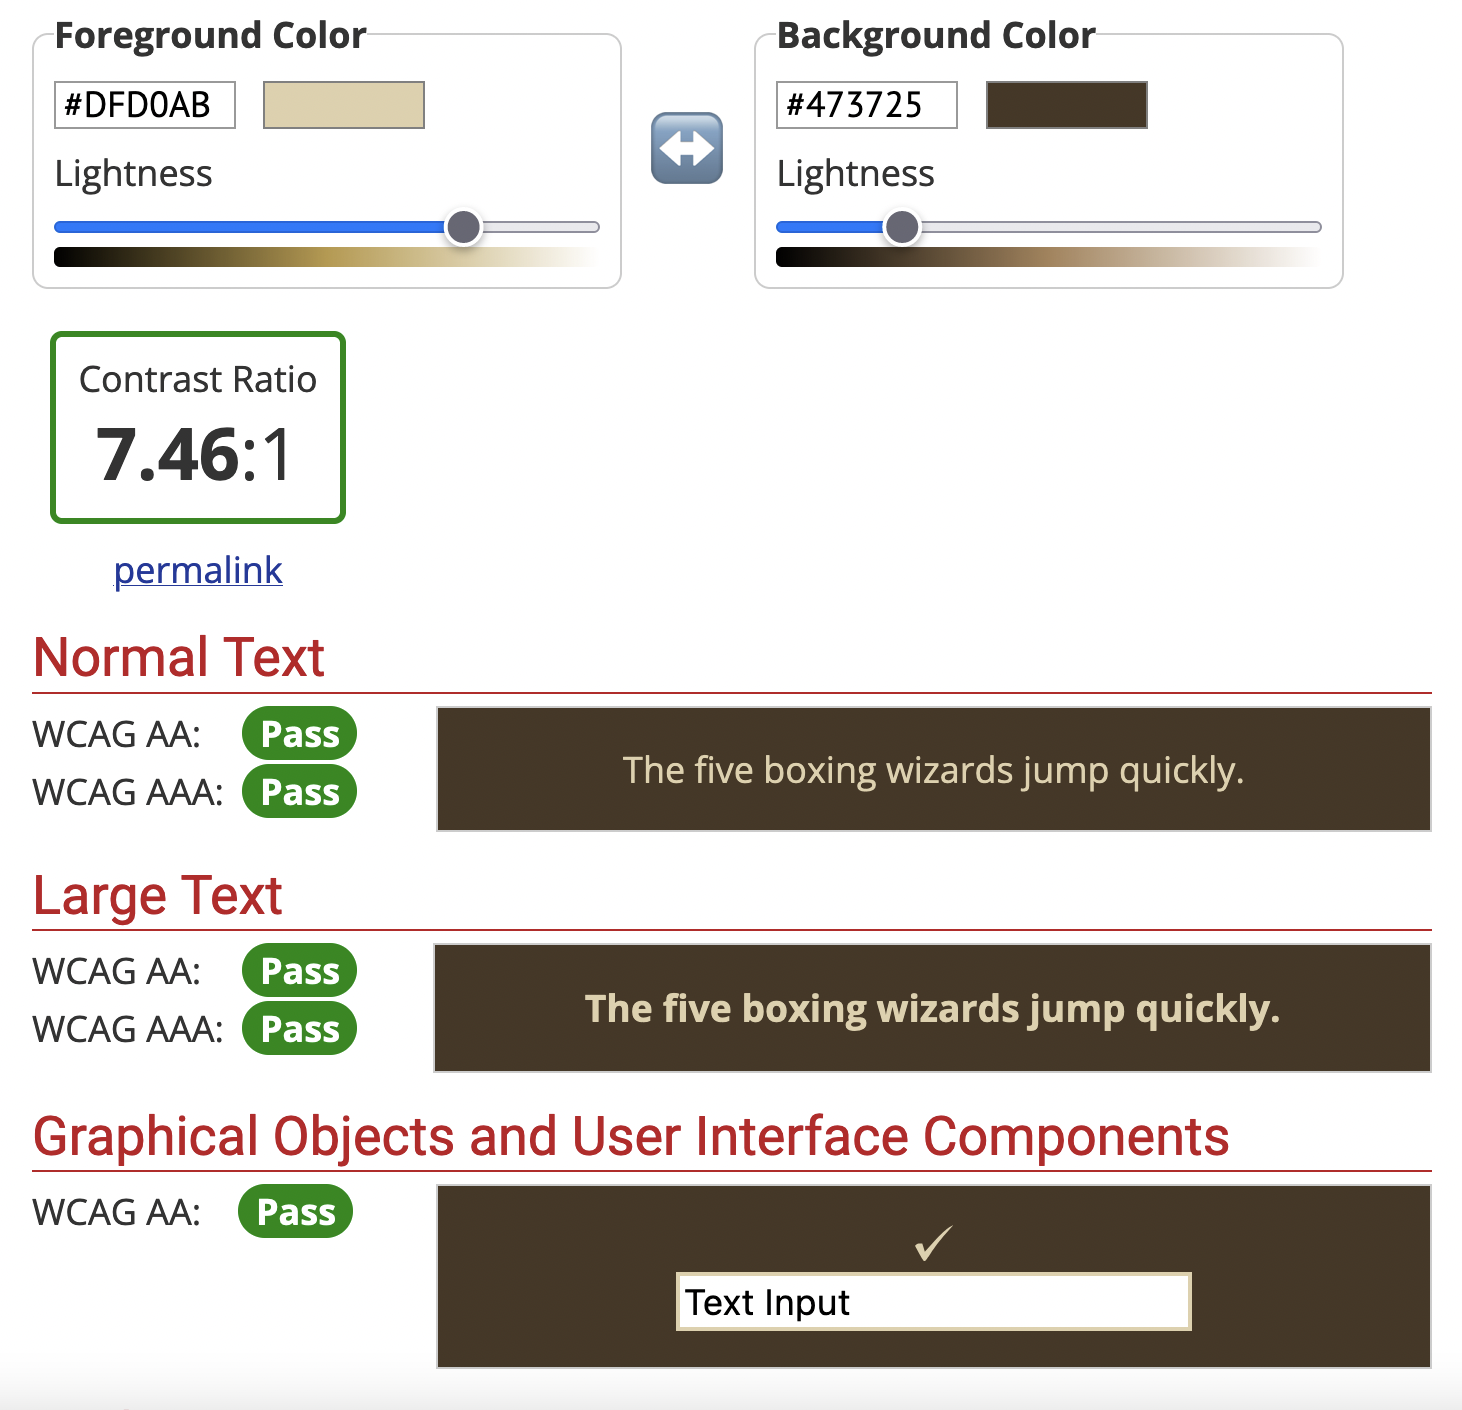
\includegraphics[scale=0.3]{immagini/controllo-colori/dark-mode/testo-principale_background-menu.png}
		\caption{Contrasto tra colore dei link del menù e il loro sfondo in modalità desktop.}
	\end{figure}

	\begin{figure}[H]
		\centering
		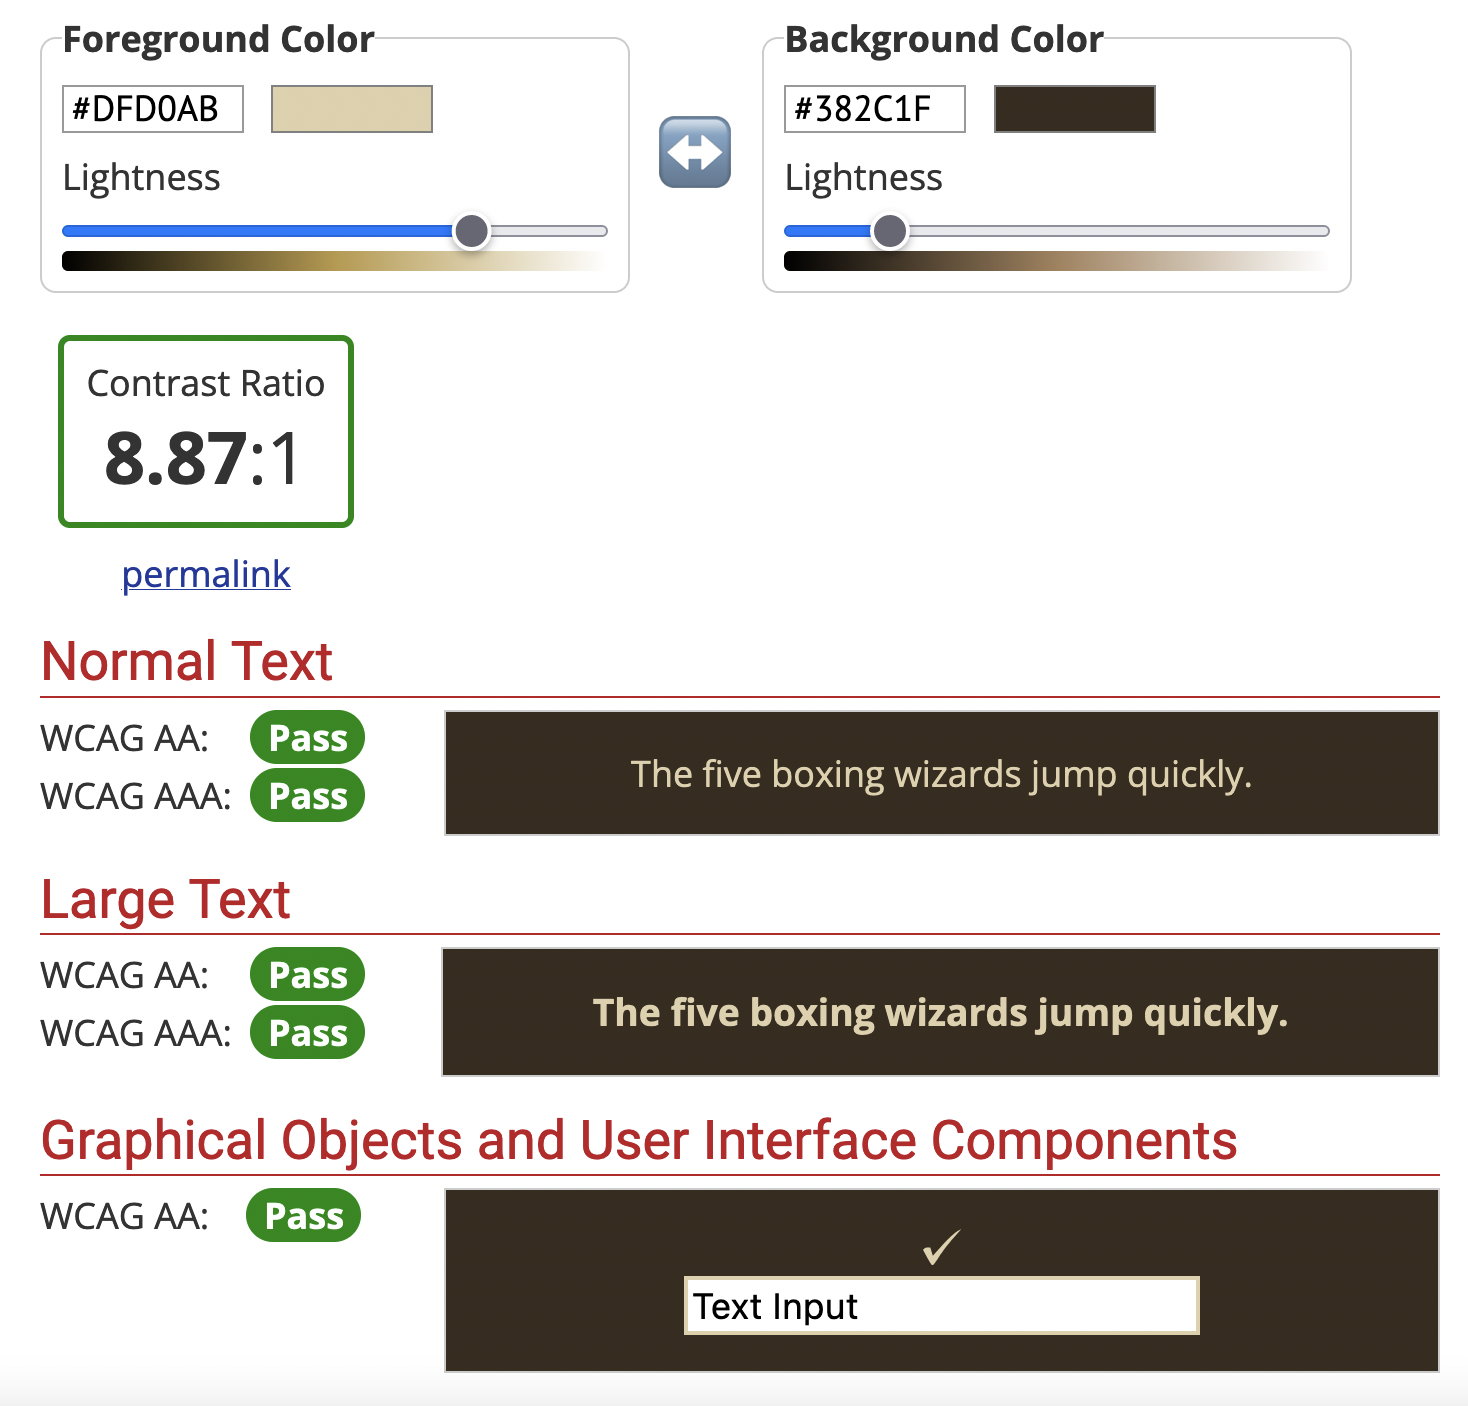
\includegraphics[scale=0.3]{immagini/controllo-colori/dark-mode/testo-principale_sfondo-article-p.png}
		\caption{Contrasto tra colore del testo principale e sfondo delle schede degli allenamenti.}
	\end{figure}

	\begin{figure}[H]
		\centering
		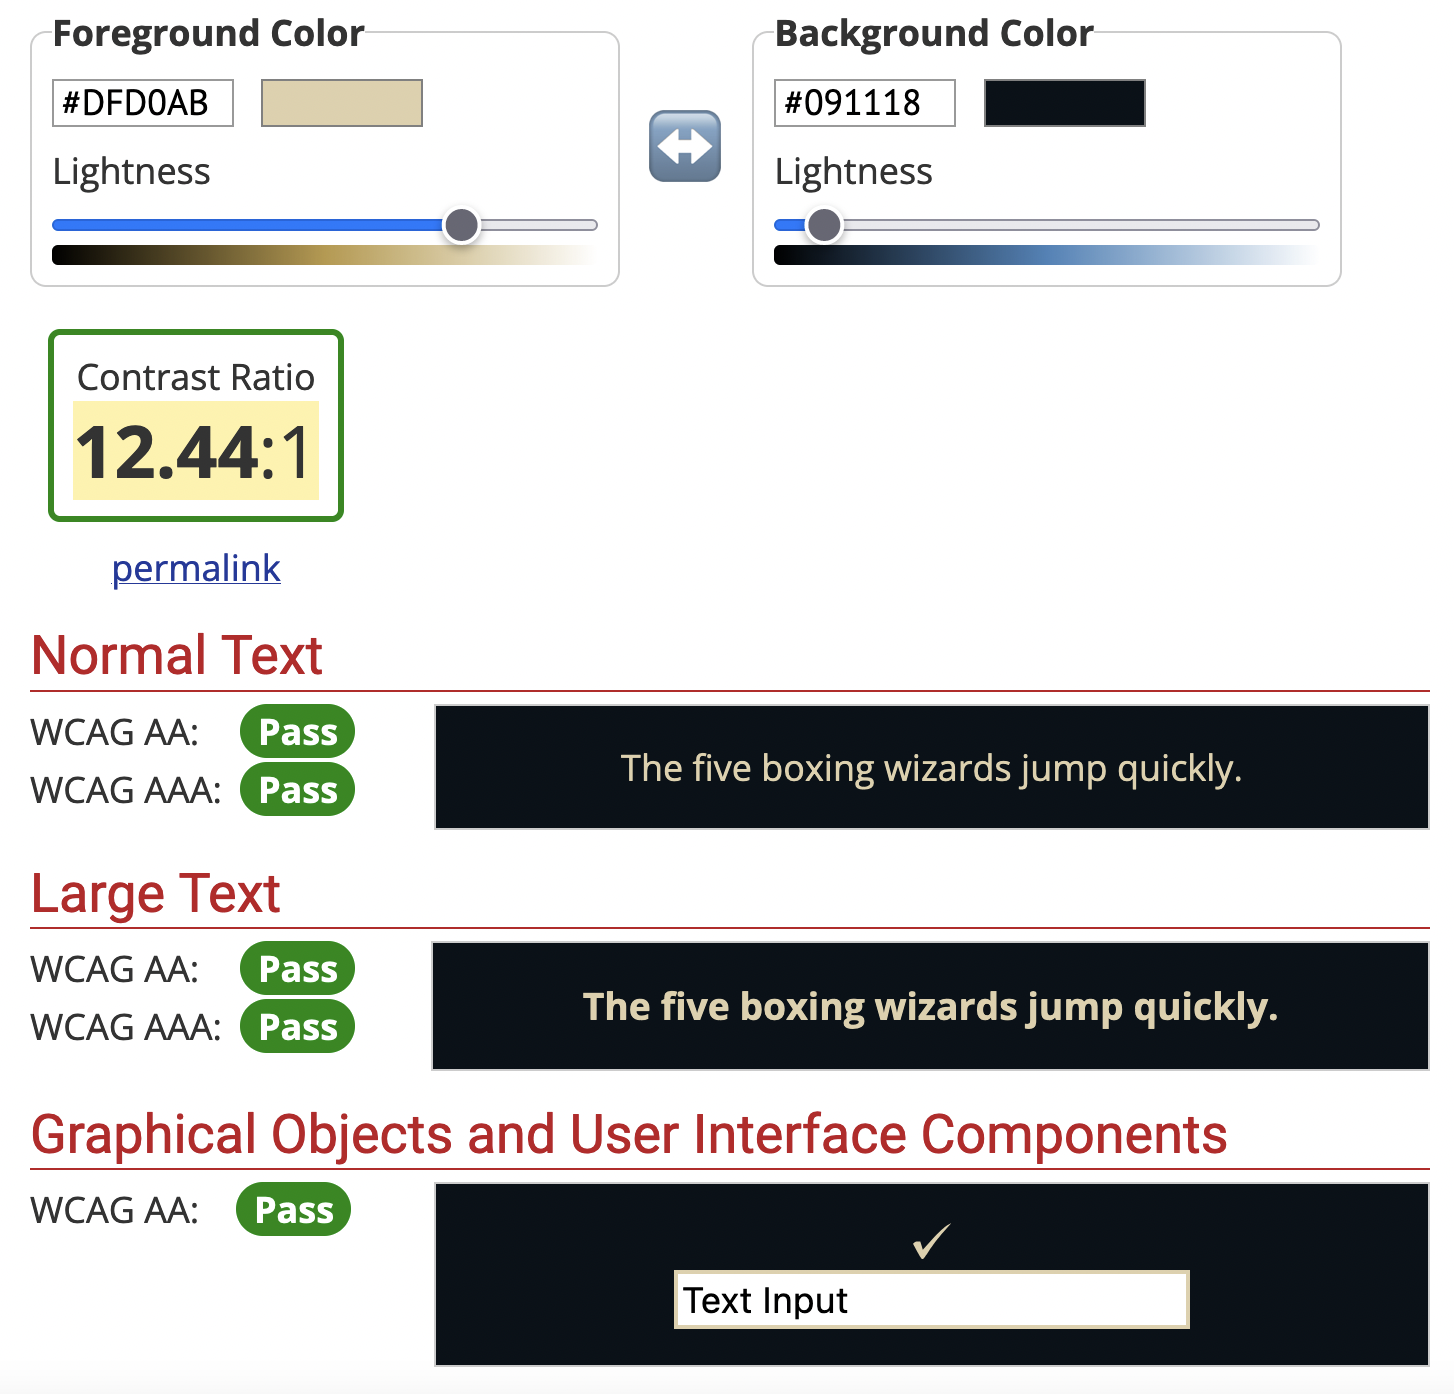
\includegraphics[scale=0.3]{immagini/controllo-colori/dark-mode/testo-principale_sfondo-div.png}
		\caption{Contrasto tra colore del testo principale e sfondo dei div.}
	\end{figure}

	\subsection{Noscript}
	Abbiamo fatto in modo che il documento Javascript definisca tutte delle funzioni di comportamento opzionali e non essenziali, come per esempio la dark-mode e la gestione del burger menù nella modalità mobile e tablet, in modo tale che la disabilitazione di Javascript non comprometta la completa funzionalità del sito, mantenendo così l'accessibilità, garantendo una trasformazione elegante. In particolare, tutti i form presenti nel sito funzionano correttamente anche in assenza di Javascript, segnalando anche gli errori negli input ma solo una volta premuto il tasto invio, prevenendo l'invio di dati invalidi al server. Javascript disabilitato poteva essere un problema per la modalità tablet e per la modalità mobile in quanto la gestione del burger menù è demandata al codice Javascript. Per risolvere il problema in questa tipologia di dispositivi, se Javascript è disabilitato viene visualizzato un altro tipo di menù, garantendo la piena funzionalità del sito web.
	
	\subsection{Tabindex}
	Per tutte le pagine è stato effettuato un controllo che tutti gli elementi di interazione fossero accessibili anche da tastiera e che l'ordine di selezione degli stessi fosse corretto, ovvero che i tabindex fossero corretti. Per un corretto ed intuitivo funzionamento dei tabindex basterebbe una buona struttura delle pagine, non dovrebbe infatti essere necessario ricorrere a specificare un ordine manuale di tabindex. Per quanto riguarda i link e tutti gli elementi di interazione del contenuto vale questa raccomandazione, mentre per la navigazione del menù si è dovuti ricorrere ad un ordine manuale. L'ordine utilizzato pone al primo posto il link per andare direttamente al contenuto e saltare la navigazione, sfruttato dagli utenti che utilizzano screen reader per evitare la lettura continua del menù. Successivamente si passa alla selezione dei link che compongono il menù, fino al link per la pagina Galleria. Poi viene selezionato il toggle per il cambio dello schema dei colori e, subito dopo, il link per l'area personale. Da quel punto in avanti viene utilizzato l'ordine di selezione automatico. Questo accorgimento si è rivelato necessario a causa della scelta di posizionare il toggle per il cambio dello schema dei colori nella barra del menù di navigazione, prima del link all'area personale.

	\section{Presentazione}
	Per quanto riguarda la presentazione, tramite CSS abbiamo implementato un design fluido e scalabile evitando il più possibile misure fisse, favorendo l'uso di misure relative o percentuali. Inoltre abbiamo utilizzato layout flex e grid che garantiscono una trasformazione elegante nella presentazione nei vari dispositivi. In particolare il layout grid lo abbiamo utilizzato nelle pagine in cui avevamo bisogno di un'interfaccia a griglia e sapevamo di avere un numero fisso di elementi da impaginare, mentre il layout flex lo abbiamo usato quando il numero di elementi da impaginare non era conosciuto a priori e quindi avevamo bisogno di un'impaginazione flessibile. Operare in questo modo, oltre a migliorare l'accessibilità, permette una corretta visualizzazione delle pagine su tutte le tipologie di dispositivi, senza impattare negativamente la navigazione tramite screen reader. Seguendo la tecnica del Responsive Web Design abbiamo prodotto tre fogli di stile differenti, uno per ogni tipologia di dispositivo: desktop, tablet, mobile.

	\subsubsection{Desktop}
	Per una descrizione dettagliata dell'header consultare la sezione \hyperref[header]{Header}, per il contenuto la sezione \hyperref[contenuto]{Contenuto}.

	\subsubsection{Tablet e Mobile}
	In merito alla visualizzazione tablet e mobile, il menù è nascosto. Per aprire il menù, basta cliccare sul burger menù in alto a sinistra, che è un elemento ormai ben conosciuto da parte degli utenti mobile e tablet. Abbiamo scelto quel posizionamento perché quell'area di schermo è la più guardata quando gli utenti cercano i link alle altre pagine ed inoltre nella maggior parte dei siti web il burger menù è posizionato nell'angolo in alto a sinistra e ciò permette al nostro sito di essere più familiare per l'utente. Per quanto riguarda l'immagine del titolo, nella modalità mobile cambia e viene sostituita da un'immagine più stretta in quanto la stessa immagine utilizzata per la modalità desktop e tablet risultava troppo larga e non ben leggibile. 


	\subsubsection{Stampa}
	Nel layout di stampa il font è di tipo serif, il testo all'interno dei paragrafi è giustificato, le dimensioni delle immagini sono ridotte e non ci sono immagini di background. Non sono visualizzati elementi come nav, footer, pulsanti non rilevanti e altri. I link interni al sito sono sottolineati e seguiti dall'url tra parentesi tonde, mentre i link esterni sono sottolineati e seguiti dall'url tra parentesi quadre. Le abbreviazioni sono seguite dal testo completo scritto tra parentesi quadre. Si è cercato, per quanto possibile, di mantenere i contenuti correlati sulla stessa pagina. Infine è stata prestata particolare attenzione al layout di stampa della pagina Dettagli allenamento per permettere all'utente di stampare la propria scheda di allenamento tramite l'apposito pulsante, la pagina infatti presenta un layout di stampa ben curato e differente da quello di tutte le altre pagine.

	\section{Comportamento}
	\subsection{Javascript}
	Per il comportamento di determinate pagine del sito, lato client, è stato utilizzato un unico file Javascript che comprende diverse funzioni, la maggior parte per far segnalare gli errori nell'input agli utenti, in quanto il controllo di integrità dei dati è demandato alle funzionalità di HTML5, per quanto riguarda i controlli lato client, assegnando i giusti attributi ai tag <input>. Proprio per questo motivo nei vari <input> abbiamo utilizzato gli attributi required, pattern, maxlength, min e max. Inoltre, usando l'attributo title, quando è presente un errore nell'input e viene inviato il form, la pagina HTML di default fa visualizzare all'utente un messaggio di errore contenente la stringa dell'attributo title. Questo rende il codice Javascript relativo alla visualizzazione dei messaggi di errore una funzionalità aggiuntiva ma non essenziale. Siccome il solo controllo di integrità dei dati lato client non è sufficiente, tutte le nostre pagine PHP che ricevono dati in input ne controllano la validità lato server e in caso di non conformità fanno visualizzare un errore.  In generale abbiamo fatto in modo che le funzioni Javascript non fossero essenziali per il completo funzionamento del sito e  infatti le nostre pagine web sono completamente fruibili con tutte le loro funzionalità anche con Javascript disabilitato.

	\subsubsection{Funzionalità}
	\begin{itemize}
		\item \textbf{initDarkMode()}: questa funzione viene chiamata in tutte le pagine del sito e serve per inizializzare lo switch della darkmode, assegnandogli all'evento click la funzione \textbf{switchTheme()} che si occupa di cambiare tema. In particolare utilizziamo localStorage per salvarci il tipo di tema impostato dall'utente, in modo tale che cambiando pagina o effettuando un nuovo accesso al sito in un momento diverso, rimanga impostato il tema utilizzato nella navigazione precedente.
		\item \textbf{addOnBlurEventInput()}: questa funzione si occupa di assegnare ai vari campi di input, se presenti, le rispettive funzioni \textbf{check\_validity\_*()} all'evento blur - ovvero quando l'elemento perde il focus - in modo tale da visualizzare un messaggio di errore appropriato per ogni campo di input.
		\item \textbf{initCounter()}: questa funzione ha il compito di inizializzare il meccanismo di chiamate AJAX per aggiornare ogni 8 secondi il contatore di persone all'interno della palestra presente nella home. In particolare viene chiamata la pagina \textbf{number\_generator.php} passandogli come parametro GET il numero attuale di persone dentro alla palestra, in modo tale da simulare un incremento o decremento del numero di persone che si stanno allenando. L'idea era di simulare un meccanismo di conteggio delle persone all'interno della palestra con l'uso di un tornello connesso al server: in pratica il valore fornito dalla pagina PHP è come se fosse quello fornito dal tornello.
		\item \textbf{initBurgermenu()}: funzione che si occupa di inizializzare gli eventi per aprire e chiudere il menù - solo per la modalità tablet e mobile - assegnando all'evento click dell'icona del burger menù la funzione \textbf{openNav()} e all'evento click dell'icona della croce per chiudere il menù la funzione \textbf{closeNav()}.
		\item \textbf{window.addEventListener-scroll}: funzione per nascondere inizialmente l'icona del torna su e farlo apparire solo quando si comincia lo scroll.
		\item \textbf{window.addEventListener-hashchange, scrollmenu()}: funzioni utili a evitare che il menù, essendo fisso, copra parte del contenuto a seguito di un link che porta verso un id specifico.
		\item \textbf{disableScadenza()}: nella modifica dei dati relativi all'abbonamento di un utente da parte di un amministratore, nella pagina Visualizza utente, quando è selezionata la voce “Nessuno” sul campo di selezione dell'abbonamento è necessario che il campo di inserimento della data di scadenza venga disattivato dinamicamente, per evitare che l'amministratore compili inutilmente il campo.
		\item \textbf{adjustGestioneUtentiHeight()}: è una funzione che viene chiamata quando, nell'area personale, l'admin decide di modificare i suoi dati personali. Serve a regolare automaticamente l'altezza massima della lista degli utenti, in modo da evitare grandi spazi bianchi sotto ai widget. Non è possibile rendere le regolazioni automatiche tramite CSS, perché è necessario impostare un'altezza massima per la lista, in modo da permettere lo scroll.
		\item \textbf{printAllenamento()}: funzione che viene assegnata all'evento click del bottone "Stampa questo allenamento" presente nella pagina di dettaglio dell'allenamento.
	\end{itemize}
	
	\subsection{PHP}
	Il comportamento del sito lato server è gestito dai file php, i quali permettono di effettuare tutte le operazioni relative al database: inserimento, cancellazione e fruizione dei dati. Il codice PHP è diviso in diversi file, uno per ogni pagina dinamica del nostro sito. Inoltre abbiamo utilizzato alcuni file php per contenere le funzioni di controllo degli input e altre funzioni di uso generico.
	\subsubsection{Validazione}
	I dati inseriti nelle form sono validati lato server con le stesse espressioni regolari utilizzate in javascript, inoltre vengono effettuati controlli che non possono essere eseguiti lato client come verificare che lo username inserito al momento della registrazione non sia già usato da un altro utente.
	\subsubsection{Sicurezza}
	Le query per interagire col database sono realizzate tramite prepared statement al fine di evitare ogni tipo di SQL Injections. Per la maggior parte dei dati immessi da un utente non è possibile inserire caratteri speciali, mentre nell'inserimento di un allenamento, dove è prevista la possibilità di inserire caratteri speciali, viene utilizzata la funzione php htmlspecialchars la quale previene ogni tipo di script injection. Per non salvare in chiaro le password all'interno del database, viene utilizzata la funzione di hashing BCRYPT.
	\subsubsection{Sessioni}
	Le variabili di sessione php utilizzate sono le seguenti:
	\begin{itemize}
		\item \$\_SESSION["loggedin"] = true se l'utente è loggato, false altrimenti.
		\item \$\_SESSION["username"] = allo username dell'utente se esso è loggato.
		\item \$\_SESSION["isAdmin"] = true se l'utente loggato è un admin, false altrimenti.
		\item \$\_SESSION["followAllenamento"] = id dell'allenamento che è stato iniziato o smesso di essere seguito.
		\item \$\_SESSION["deleted"] = true se è appena stato eliminato un allenamento.
		\item \$\_SESSION["followChange"] = true se un allenamento visualizzato nel dettaglio è stato iniziato o smesso di essere seguito.

	\end{itemize}
	\subsubsection{Classe DBAccess}
	Questa classe viene utilizzata da tutte le pagine PHP che necessitano di reperire dati in modo dinamico, e pertanto dal database. Ne semplifica l'interazione e permette il riuso di codice. Possiede tutte le credenziali per accedervi e mette a disposizione funzionalità per aprire e chiudere la connessione, eseguire query in lettura e scrittura. Garantisce un adeguato livello di sicurezza evitando SQL Injections tramite i prepared statement. Inoltre dealloca i risultati delle query per migliorare l'efficienza. Durante la realizzazione del sito è stato usato per ogni membro un file di configurazione contenente le credenziali necessari alla classe per la connessione. Questa procedura permette di usare la stessa classe e accedere a database diversi senza modificare ogni volta i valori preimpostati. Per la consegna questo meccanismo è stato rimosso e sono state inserite direttamente nella classe le credenziali di chi consegna.

	\section{Fase di test}
	\subsection{Validazione}
	Tutte le pagine html e i file css sono stati sottoposti alla validazione tramite l'uso dei tool descritti nella sezione relativa alla realizzazione.
	
	\subsection{Peso}
	Il peso di ogni pagina del sito è stato calcolato tramite lo strumento descritto nella sezione relativa alla realizzazione. Tutte le pagine eccetto la galleria (3.4 MB) non superano 1 MB di peso, non è stato possibile alleggerire il peso della galleria senza perdita di qualità delle immagini.
	
	\subsection{Browser e dispositivi}
	Il sito è stato testato direttamente sui seguenti sistemi operativi:
	\begin{itemize}
		\item Windows 10
		\item Windows 11
		\item macOS
		\item Linux
		\item Android 11
		\item IOS 15
	\end{itemize}
	Il sito è stato testato direttamente sui seguenti browser:
	\begin{itemize}
		\item Chrome v97
		\item Firefox v96
		\item Safari v15.2 (i file CSS sono direttamente nella root altrimenti questo browser non riesce ad accedere alle variabili CSS)
		\item Edge v97
		\item Opera v83
		\item Internet explorer 21h1
		\item Lynx v2.8.9
	\end{itemize}   

	\section{Organizzazione del gruppo}
	\subsection{Processo di sviluppo}
	Abbiamo iniziato scegliendo un dominio applicativo adatto ad un sito web che potesse rispettare tutti i vincoli del progetto e che fosse d'interesse a ogni membro del gruppo. Siamo quindi passati alla sua progettazione definendo in dettaglio componenti e funzionalità. Definita la struttura base delle pagine, abbiamo suddiviso e assegnato le pagine HTML e il relativo CSS tra i vari membri. Successivamente è stata realizzata la parte in PHP con lo stesso metodo citato precedentemente: definita la classe per la connessione al database, abbiamo suddiviso e assegnato le pagine PHP e il relativo CSS tra i vari membri. In seguito sono state realizzate le funzioni JavaScript, seguito dal CSS mobile e di stampa. Infine abbiamo proceduto a verificare la separazione del sito, l'accessibilità e i test. Tra ogni fase è seguita una fase di unione dei lavori, sistemazione dei conflitti ed errori minori. Abbiamo concluso scrivendo la relazione.
	
	\subsection{Divisione del lavoro}

	\subsubsection{Adnan Latif Gazi}
	\begin{itemize}
		\item Pagine HTML di Trainers, Home, 404 e 500;
		\item CSS desktop;
		\item Database;
		\item Pagine PHP di Allenamenti, Dettagli Allenamenti;
		\item Funzionalità JavaScript torna su;
		\item Verifica separazione sito, accessibilità e validazione.
	\end{itemize}

	\subsubsection{Alberto Lazari}
	\begin{itemize}
		\item Pagine HTML di Abbonati e Home;
		\item CSS desktop e mobile, in particolare delle pagine Abbonati e di Area Personale. Correzioni finali e piccoli aggiustamenti \item relativi al CSS di varie pagine ed elementi;
		\item Pagine PHP di Area personale [Admin] e visualizza-utente.php. Correzioni e refactoring codice della pagina area-personale.php;
		\item Piccoli elementi di comportamento in JavaScript;
		\item Verifica divisione sito, accessibilità e validazione;
		\item Verifica tabindex e aggiustamenti.
	\end{itemize}

	\subsubsection{Marco Andrea Limongelli}
	\begin{itemize}
		\item Pagine HTML di Attrezzature, Galleria e Home;
		\item CSS desktop e mobile;
		\item Pagine PHP di Area personale, Compra abbonamento e Conferma Acquisto Abbonamento;
		\item Funzionalità JavaScript Dark Mode, Burger Menù e visualizzazione errori negli input;
		\item Verifica divisione sito, accessibilità e validazione.    
	\end{itemize}

	\subsubsection{Francesco Protopapa}
	\begin{itemize}
		\item Pagine HTML di Storia e Home;
		\item CSS desktop, mobile e stampa
		\item Pagine PHP di Autenticazione (Accesso e Registrazione), Modifica allenamento e Inserimento allenamento;
		\item Piccoli elementi di comportamento in JavaScript;
		\item Verifica divisione sito, accessibilità e validazione.       
	\end{itemize}

\end{document}